\documentclass[11pt,a4paper]{article}
\usepackage[T1]{fontenc}
\usepackage[utf8]{inputenc}
\usepackage{lmodern,microtype}
\usepackage[margin=2.5cm]{geometry}
\usepackage{amsmath,amssymb,graphicx,float,booktabs,longtable,adjustbox,seqsplit,hanging}
\usepackage[font=small,labelfont=bf]{caption}
\usepackage{xcolor,titlesec,fancyhdr,parskip,listings}
\usepackage{xurl,CJKutf8}
\usepackage[hidelinks]{hyperref}
\definecolor{navy}{HTML}{1F3A5F}
\titleformat{\section}{\Large\bfseries\color{navy}}{\thesection}{0.8em}{}
\titleformat{\subsection}{\large\bfseries\color{navy}}{\thesubsection}{0.8em}{}
\setlength{\headheight}{14pt}
\pagestyle{fancy}
\fancyhf{}
\lhead{\small Bitcoin Price Forecasting with ARIMA}
\rhead{\small AHAMED MD SAJIB (2026250206)}
\cfoot{\thepage}
\lstset{language=Python,basicstyle=\ttfamily\scriptsize,breaklines=true,columns=fullflexible,
  keepspaces=true,showstringspaces=false,frame=single,keywordstyle=\color{navy}\bfseries,
  commentstyle=\color{gray}}
\hypersetup{pdftitle={Forecasting the Seven-Day Price Movement of Bitcoin with ARIMA},pdfauthor={AHAMED MD SAJIB}}
\begin{document}
\begin{titlepage}
\centering
\vspace*{0.5cm}
{\color{navy}\Huge\bfseries ASSIGNMENT\par}
\vspace{0.8cm}
{\color{navy}\rule{\linewidth}{1.2pt}}\\[0.6cm]
{\large\bfseries Topic\par}
\vspace{0.3cm}
{\color{navy}\LARGE\bfseries Forecasting the Seven-Day Price Movement\\[0.2cm] of Bitcoin with ARIMA\par}
\vspace{0.4cm}
{\color{navy}\rule{\linewidth}{1.2pt}}
\vfill
{\large\bfseries\color{navy} Submitted To\par}
\vspace{0.4cm}
{\Large \begin{CJK}{UTF8}{mj}정명애\end{CJK} (Professor)\par}
\vfill
{\large\bfseries\color{navy} Submitted By\par}
\vspace{0.4cm}
{\large\renewcommand{\arraystretch}{1.5}
\begin{tabular}{rl}
\textbf{Student name:} & AHAMED MD SAJIB \\
\textbf{Student ID:} & 2026250206 \\
\textbf{University:} & Eulji University \\
\textbf{Department:} & Global Big Data \& Artificial Intelligence \\
\textbf{Submission date:} & 27 November 2026 \\
\end{tabular}\par}
\vfill
{\color{navy}\LARGE\bfseries EULJI UNIVERSITY\par}
\end{titlepage}
\pagenumbering{roman}
\tableofcontents
\clearpage
\listoffigures
\listoftables
\clearpage
\pagenumbering{arabic}


\section*{Abstract}
\addcontentsline{toc}{section}{Abstract}

This study forecasts the Bitcoin market price for seven days using 366 daily observations from Blockchain.com covering 2025-11-25 to 2026-11-25. Over this window the price moved from \$88,276.26 to \$59,742.21 (-32.3\%), with annualised return volatility of 44.4\%. Unit-root tests support one difference of the log price (d = 1). A grid of 128 ARIMA specifications was searched on the first 292 observations, and a shortlist was compared by rolling-origin validation inside the training sample. After residual and root-admissibility screening, the selected model was ARIMA(0, 1, 0), a random walk without drift. On 74 unseen observations it gave a one-step MAPE of 1.51\% and RMSE of \$1,651.44. These figures are identical to those of the naive forecast because the two methods are mathematically the same. The forecast for 2026-11-26 to 2026-12-02 is therefore flat at \$59,742.21 (classified Neutral), with a 95\% interval on the seventh day of \$52,943.75 to \$67,413.66. The analysis finds no reliable evidence that past prices alone predict the direction of Bitcoin over this horizon. It is not investment advice.

\clearpage

\section{Introduction}

Bitcoin is a decentralised digital asset that trades continuously and is known for large price swings. Short-horizon forecasting is attractive but difficult: if prices rapidly incorporate available information, past prices should contain little exploitable information about future changes (Fama, 1970). Studies of exchange rates have shown that a random walk can be a demanding benchmark for structural and time-series models (Meese and Rogoff, 1983). Financial returns also commonly show heavy tails and volatility clustering (Cont, 2001).

The autoregressive integrated moving average (ARIMA) family, developed in the Box-Jenkins tradition (Box et al., 2015), is a transparent linear framework for modelling serial dependence. This report applies it end to end and judges it against simple benchmarks, so that apparent accuracy is not mistaken for predictive skill.

\section{Problem Statement}

The assessment task is to predict the price movement of Bitcoin for the next seven days from the past year of historical prices, using ARIMA in Python. The analytical question is whether a linear model of past daily prices indicates a direction and size of movement that can be distinguished from random fluctuation.

\section{Research Objectives}

\begin{enumerate}
  \item Obtain and validate one year of daily Bitcoin market-price data from a documented source.
  \item Describe the trend, return distribution and volatility of the series.
  \item Determine the differencing order from statistical evidence.
  \item Identify, compare and diagnose candidate ARIMA models without using test data for selection.
  \item Evaluate out-of-sample accuracy against naive, drift and moving-average benchmarks.
  \item Produce a seven-day forecast with 95\% prediction intervals and interpret its uncertainty.
\end{enumerate}

\section{Dataset Description and Data Source}

The data come from the Blockchain.com chart shown at \url{https://www.blockchain.com/ko/charts/market-price}. They were retrieved from the official chart-data API behind that chart (not scraped from the web page) on 2026-11-25 05:11:32 UTC, using the request \url{https://api.blockchain.info/charts/market-price?timespan=1year&format=json&sampled=false}. The API names the metric `Market Price (USD)' and defines it as: `Average USD market price across major bitcoin exchanges.' Values are in USD with a period of one day. The API response does not state which exchanges or weights are used. The unmodified response and the CSV file bitcoin\_historical\_data.csv are preserved; the CSV SHA-256 checksum is {\ttfamily\seqsplit{247e3fa4cf7763584543337cc004507351c8f6bbb1a6201fe023f785d99829d4}}.

As an independent plausibility check (not used in modelling), the series was compared with Coinbase BTC-USD daily closes. A Blockchain.com value stamped day D differs from the Coinbase close of day D-1 by 0.020\% on average (maximum 0.13\%, 297 days), against 1.64\% when the same dates are matched. This indicates, although the API does not document it, that each stamp behaves like a price at 00:00 UTC. Forecast dates below follow the same convention.

\begin{table}[H]
\centering
\caption{First and last five observations}
\small
\setlength{\tabcolsep}{4pt}
\begin{adjustbox}{max width=\linewidth}
\begin{tabular}{lrr}
\toprule
\textbf{Position} & \textbf{Date} & \textbf{Market price} \\
\midrule
First five & 2025-11-25 & \$88,276.26 \\
First five & 2025-11-26 & \$87,330.85 \\
First five & 2025-11-27 & \$90,517.55 \\
First five & 2025-11-28 & \$91,305.47 \\
First five & 2025-11-29 & \$90,915.26 \\
Last five & 2026-11-21 & \$58,786.67 \\
Last five & 2026-11-22 & \$60,088.31 \\
Last five & 2026-11-23 & \$61,081.74 \\
Last five & 2026-11-24 & \$61,214.41 \\
Last five & 2026-11-25 & \$59,742.21 \\
\bottomrule
\end{tabular}
\end{adjustbox}
\end{table}

\begin{table}[H]
\centering
\caption{Data validation summary}
\small
\setlength{\tabcolsep}{4pt}
\begin{adjustbox}{max width=\linewidth}
\begin{tabular}{lr}
\toprule
\textbf{Property} & \textbf{Result} \\
\midrule
Observations & 366 \\
Date range & 2025-11-25 to 2026-11-25 \\
Missing values & 0 \\
Missing calendar dates & 0 \\
Duplicate dates & 0 \\
Non-positive values & 0 \\
Data types & date: datetime; price: float64; raw timestamp: integer \\
\bottomrule
\end{tabular}
\end{adjustbox}
\end{table}

\section{Methodology}

Let P(t) denote the price on day t and y(t) its natural logarithm. The log transform makes changes proportional, moderates scale-dependent variance and guarantees positive forecasts. With B the backshift operator, an ARIMA(p, d, q) model is

\begin{equation}
\phi(B)\,(1-B)^d\,y_t = c + \theta(B)\,\varepsilon_t
\end{equation}

\begin{equation}
\begin{gathered}
\phi(B)=1-\phi_1B-\cdots-\phi_pB^p,\\ \theta(B)=1+\theta_1B+\cdots+\theta_qB^q
\end{gathered}
\end{equation}

where the errors are assumed to be white noise (Gaussian for likelihood and interval calculations). Parameters were estimated by exact maximum likelihood in statsmodels (Seabold and Perktold, 2010). A constant in a once-differenced model represents drift. Because forecasts are made on the log scale, the exponentiated point forecast is the conditional median of price. Under log-normality the conditional mean is higher:

\begin{equation}
\begin{gathered}
\hat P^{\,med}_{T+h}=e^{\hat y_{T+h}},\\ \hat P^{\,mean}_{T+h}=e^{\hat y_{T+h}+\hat\sigma_h^2/2}
\end{gathered}
\end{equation}

\begin{equation}
95\%\ \mathrm{interval}:\ \exp(\hat y_{T+h}\pm 1.96\,\hat\sigma_h)
\end{equation}

The intervals reflect future-error variance under the fitted model. They do not include uncertainty about which model is correct or, in the standard state-space calculation, parameter estimation uncertainty.

\section{Data Preprocessing}

Unix timestamps were converted to UTC dates, observations sorted chronologically, and prices checked to be numeric and positive. Duplicate dates would be resolved by keeping the latest timestamp. The series was re-indexed to a complete daily calendar. The declared rule for any gap was forward filling, which uses only past information and therefore avoids look-ahead leakage. No duplicates, gaps or invalid values were found, so no observation was altered or filled. Outliers were retained because extreme moves are genuine features of the market and removing them would understate risk.

\section{Exploratory Data Analysis}

\begin{table}[H]
\centering
\caption{Descriptive statistics}
\small
\setlength{\tabcolsep}{4pt}
\begin{adjustbox}{max width=\linewidth}
\begin{tabular}{lrrr}
\toprule
\textbf{Statistic} & \textbf{Price (USD)} & \textbf{Daily change (USD)} & \textbf{Daily return (\%)} \\
\midrule
count & 366.00 & 365.00 & 365.00 \\
mean & 75,265.68 & -78.18 & -0.08 \\
std & 9,752.10 & 1,713.46 & 2.33 \\
min & 58,534.28 & -10,192.12 & -13.96 \\
25\% & 65,986.24 & -1,015.73 & -1.39 \\
50\% & 75,802.58 & -32.03 & -0.04 \\
75\% & 82,145.99 & 710.57 & 0.93 \\
max & 96,931.94 & 7,708.26 & 12.27 \\
skewness & 0.21 & -0.14 & 0.07 \\
excess kurtosis & -1.09 & 4.97 & 5.90 \\
\bottomrule
\end{tabular}
\end{adjustbox}
\end{table}

\begin{figure}[H]
\centering
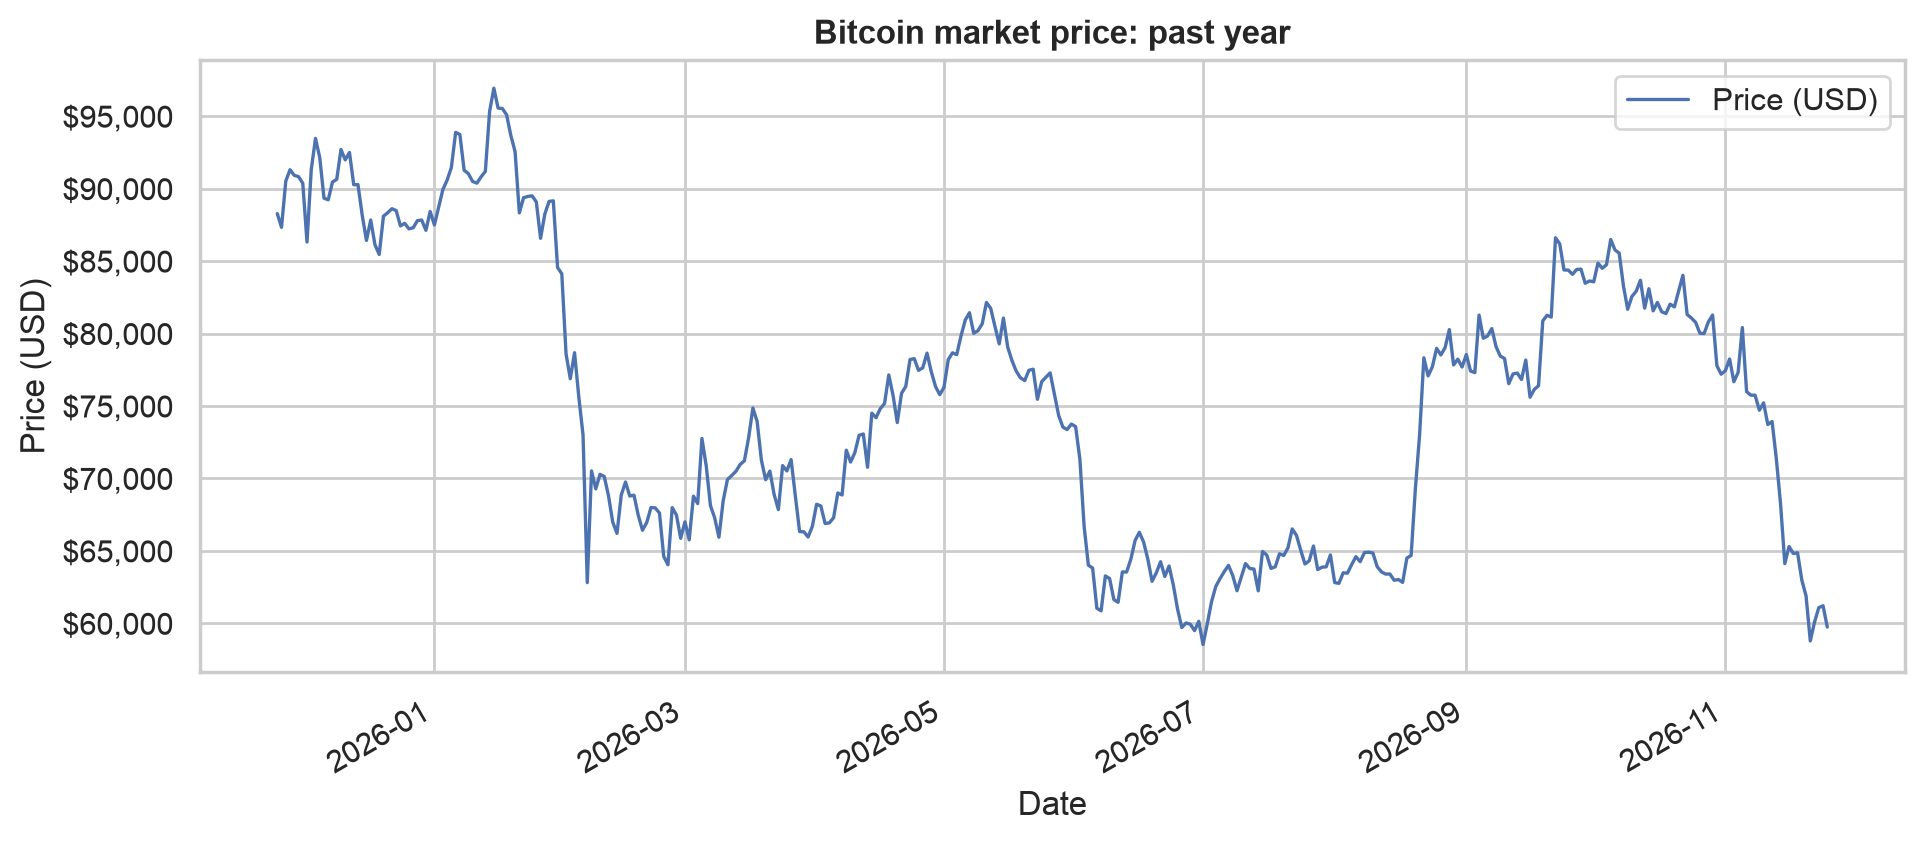
\includegraphics[width=\linewidth,height=0.78\textheight,keepaspectratio]{figures/historical_price.png}
\caption{Daily Bitcoin market price over the past year}
\end{figure}

The series is not level around a constant mean. The maximum was \$96,931.94 on 2026-01-15 and the minimum \$58,534.28 on 2026-07-01; the largest peak-to-trough decline was 39.6\%. Visible phases include a sharp fall from late January to early February 2026, a recovery to May, a decline in early June, a rapid rise in late August, and a pronounced fall in November. These are descriptions of the price path; this study does not analyse their causes.

\begin{figure}[H]
\centering
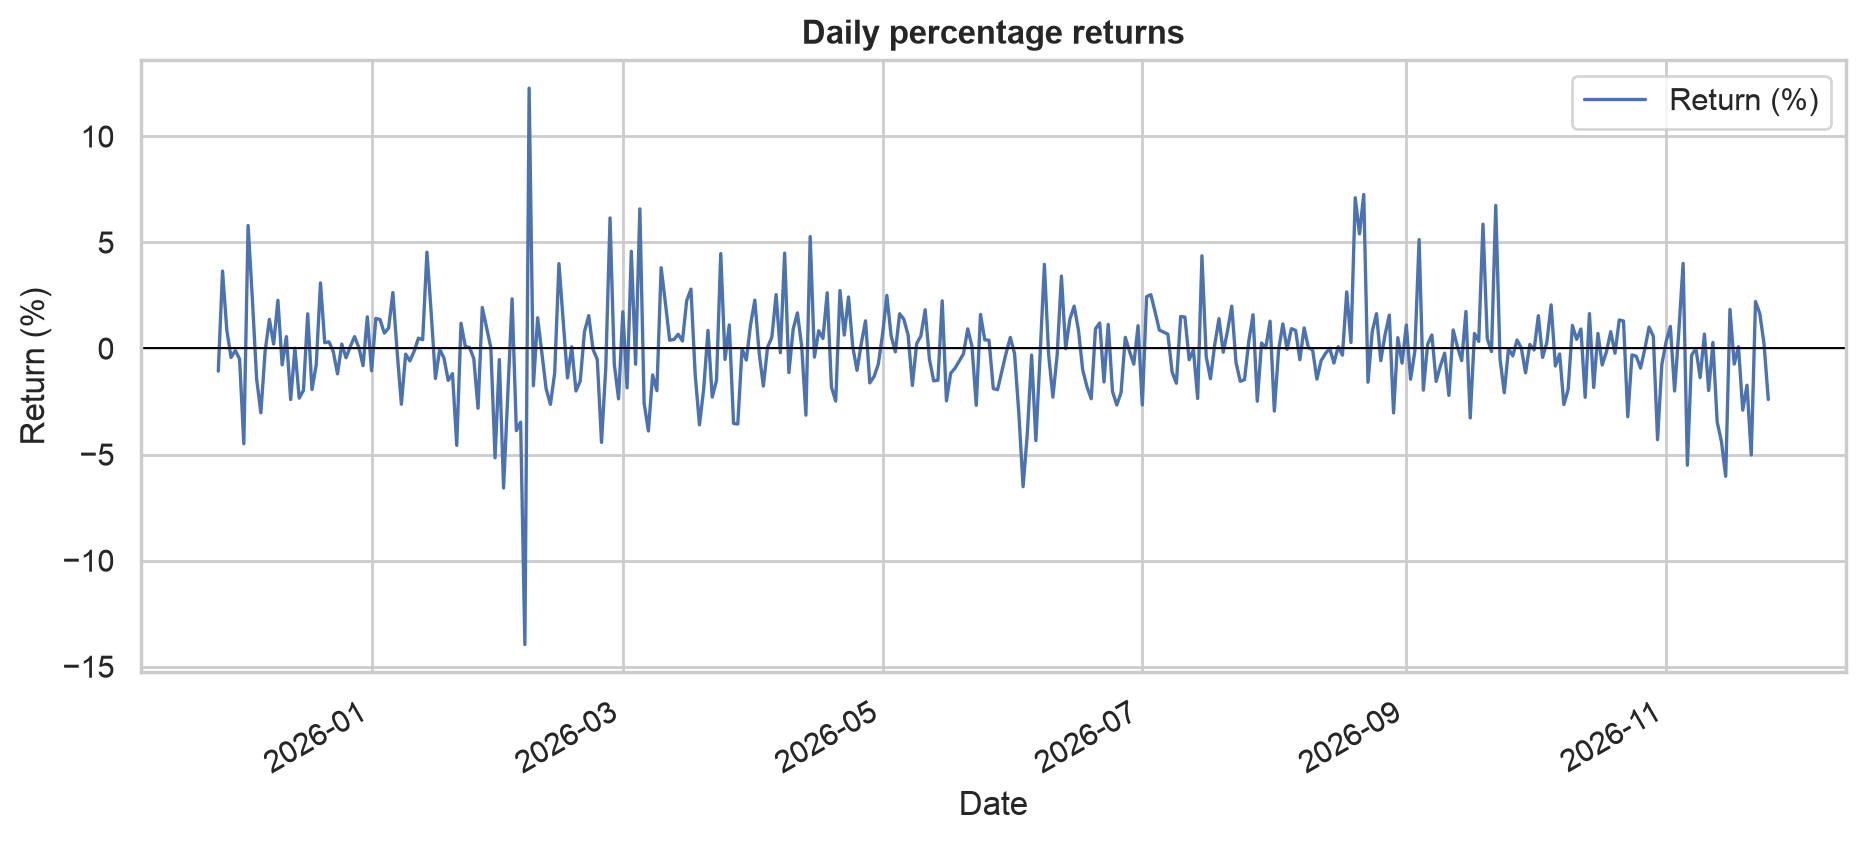
\includegraphics[width=\linewidth,height=0.78\textheight,keepaspectratio]{figures/daily_returns.png}
\caption{Daily percentage returns}
\end{figure}

Mean daily return was -0.080\% with standard deviation 2.33\%. There were 176 rising and 189 falling days. The largest fall was -13.96\% (2026-02-06) and the largest gain 12.27\% (2026-02-07), on consecutive days. Excess kurtosis of 5.90 shows far heavier tails than a normal distribution, and large moves appear in clusters.

\begin{figure}[H]
\centering
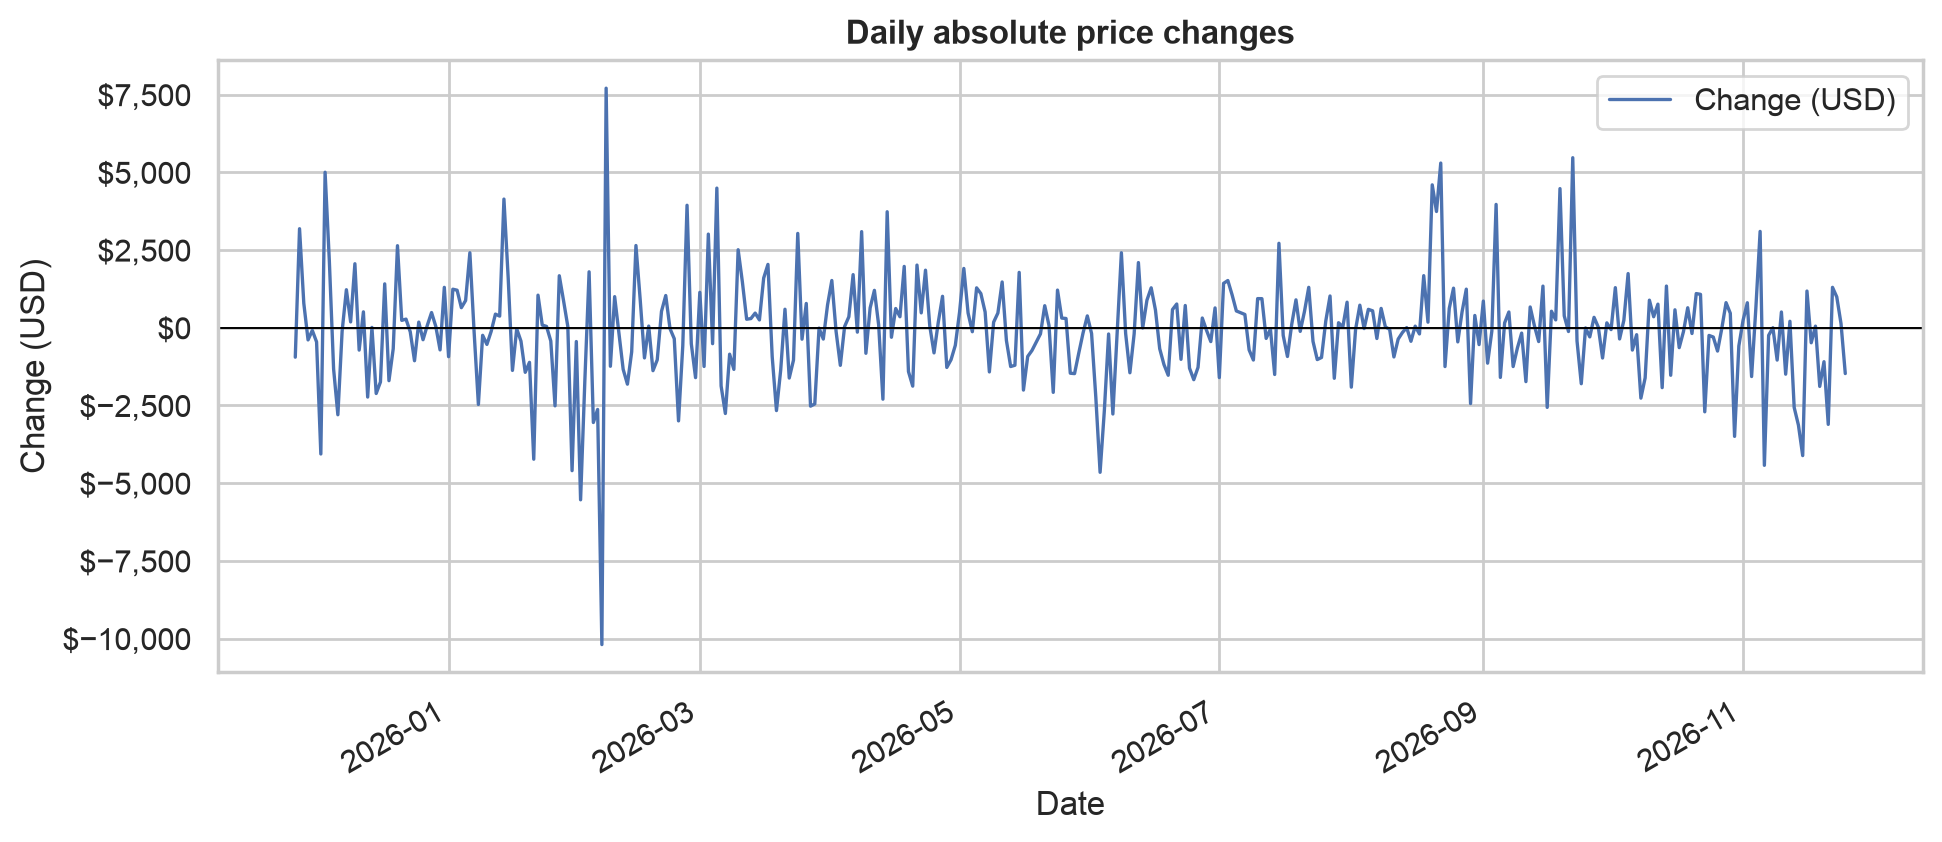
\includegraphics[width=\linewidth,height=0.78\textheight,keepaspectratio]{figures/daily_changes.png}
\caption{Daily absolute price changes}
\end{figure}

Absolute changes tell the same story in dollars: quiet stretches are interrupted by bursts of several thousand dollars per day. Because a given percentage move is worth more dollars at a higher price, the log scale is preferred for modelling.

\begin{figure}[H]
\centering
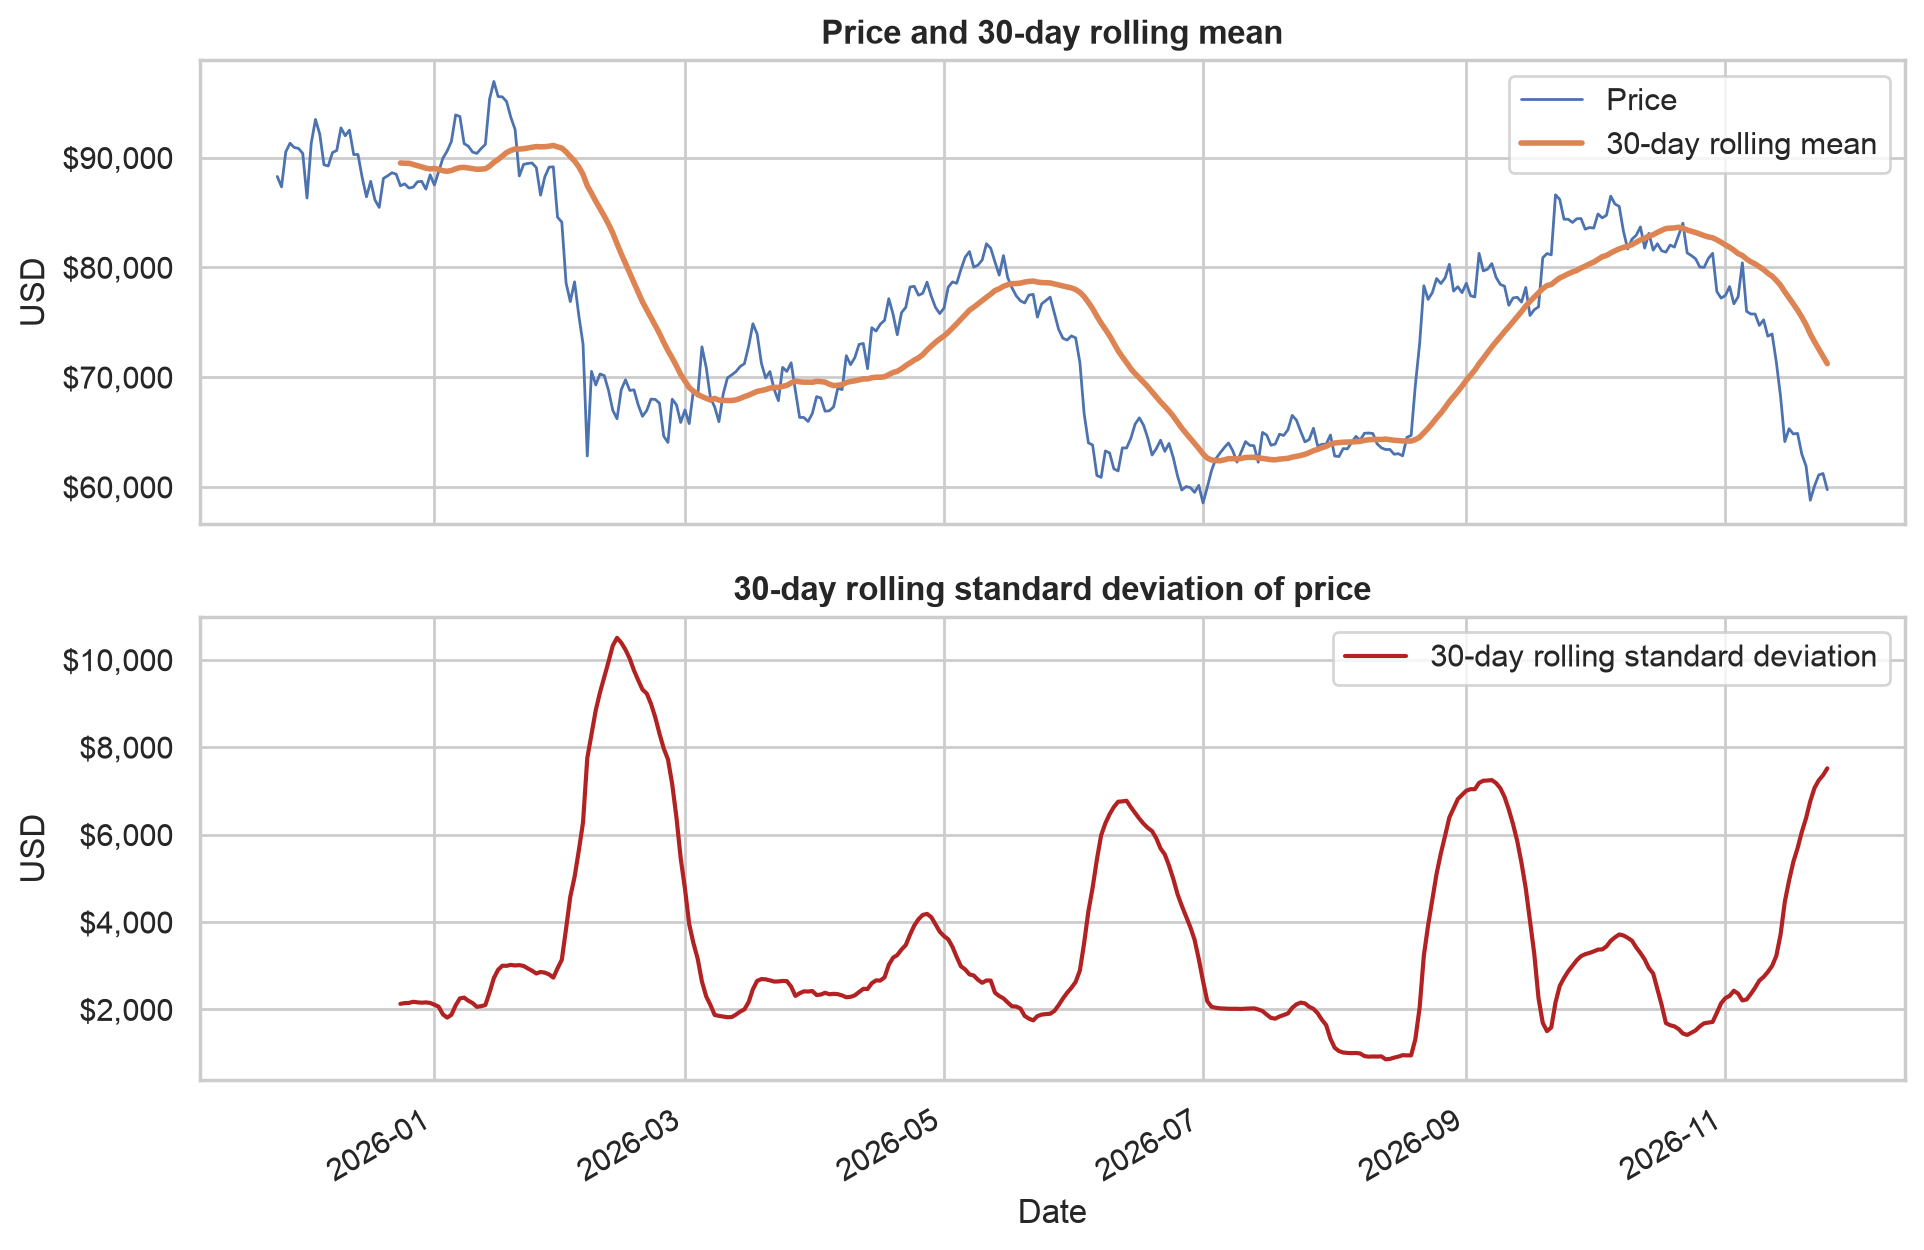
\includegraphics[width=\linewidth,height=0.78\textheight,keepaspectratio]{figures/rolling_statistics.png}
\caption{30-day rolling mean and rolling standard deviation}
\end{figure}

The rolling mean drifts substantially and lags turning points. The rolling standard deviation ranged from \$858.63 (2026-08-13) to \$10,499.92 (2026-02-13). It measures dispersion of price levels, so it rises during trends as well as during erratic trading. Both statistics change over time, which is evidence against stationarity.

\begin{figure}[H]
\centering
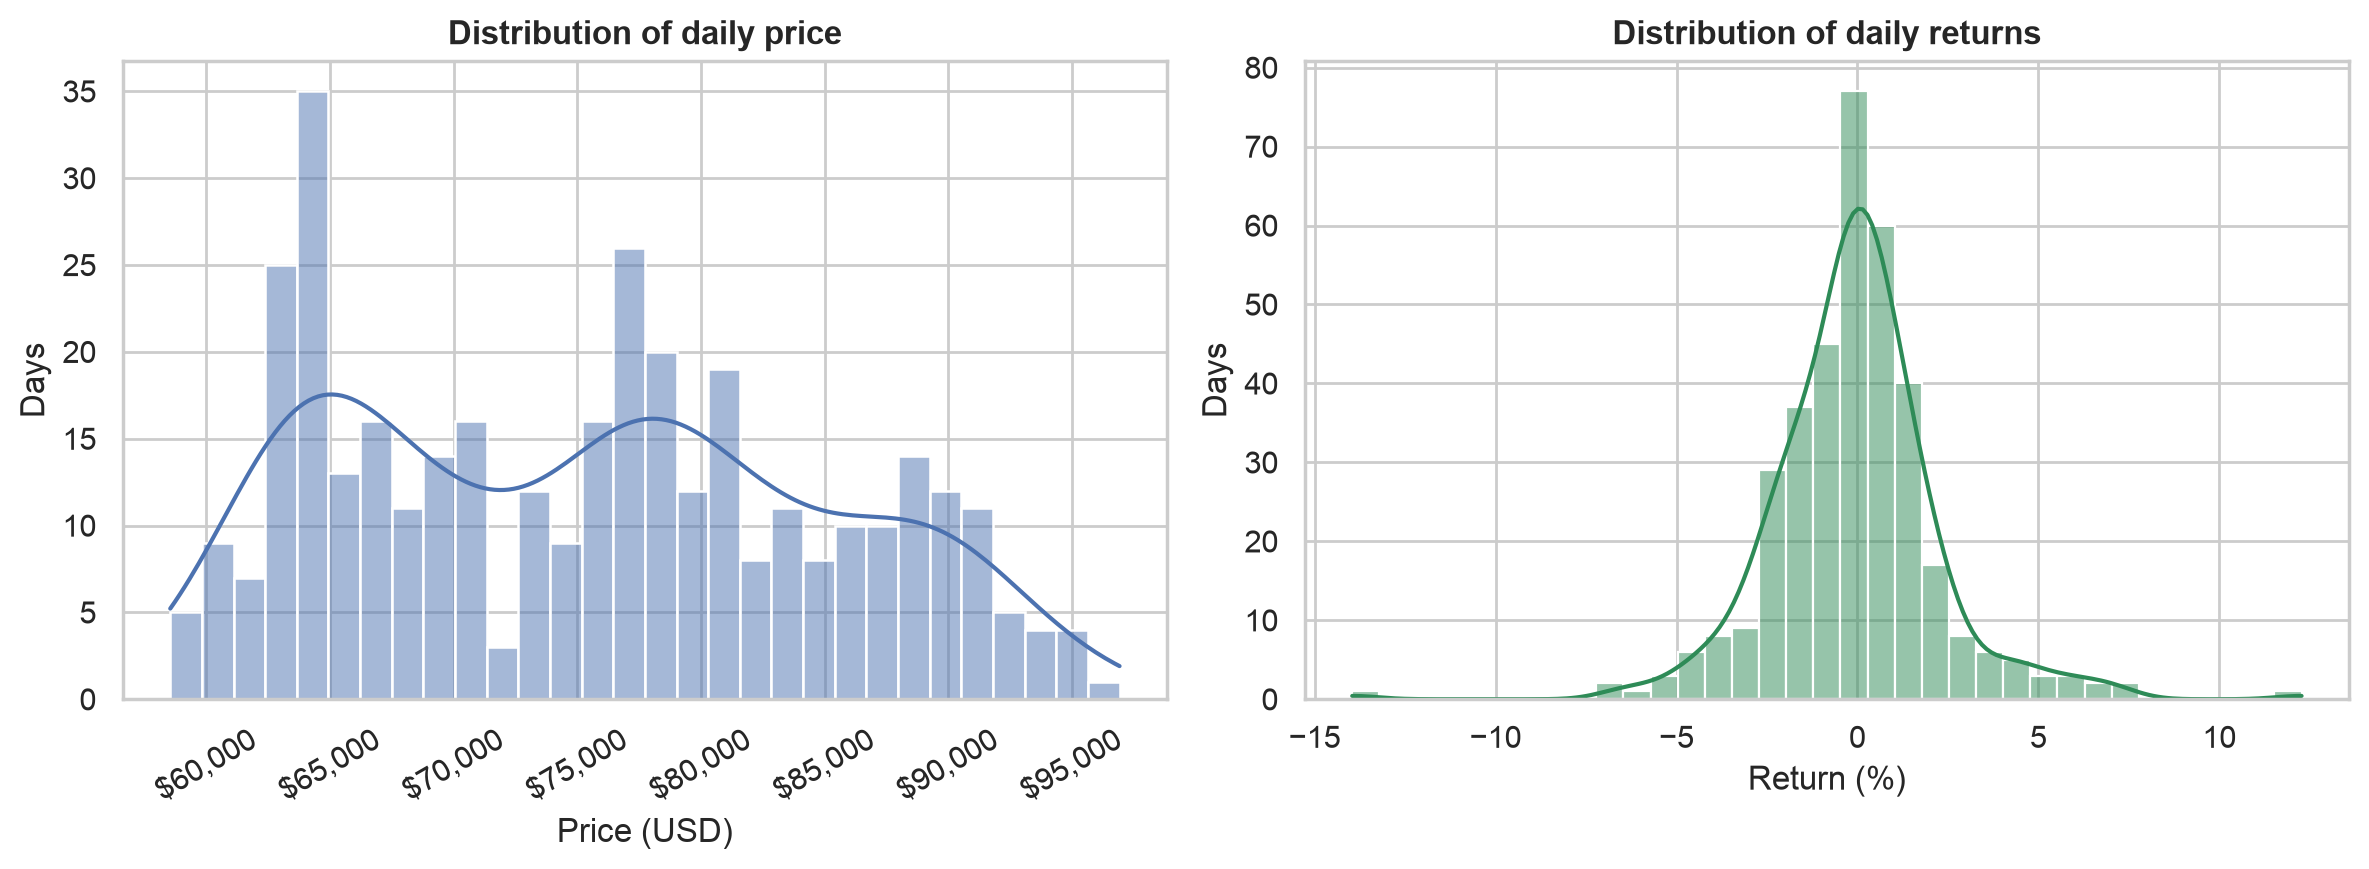
\includegraphics[width=\linewidth,height=0.78\textheight,keepaspectratio]{figures/price_distribution.png}
\caption{Distribution of daily prices and daily returns}
\end{figure}

The price histogram has several clusters that correspond to different market phases; it describes time spent at each level and should not be read as a stable probability distribution. Returns are centred near zero, sharply peaked and heavy-tailed.

\begin{figure}[H]
\centering
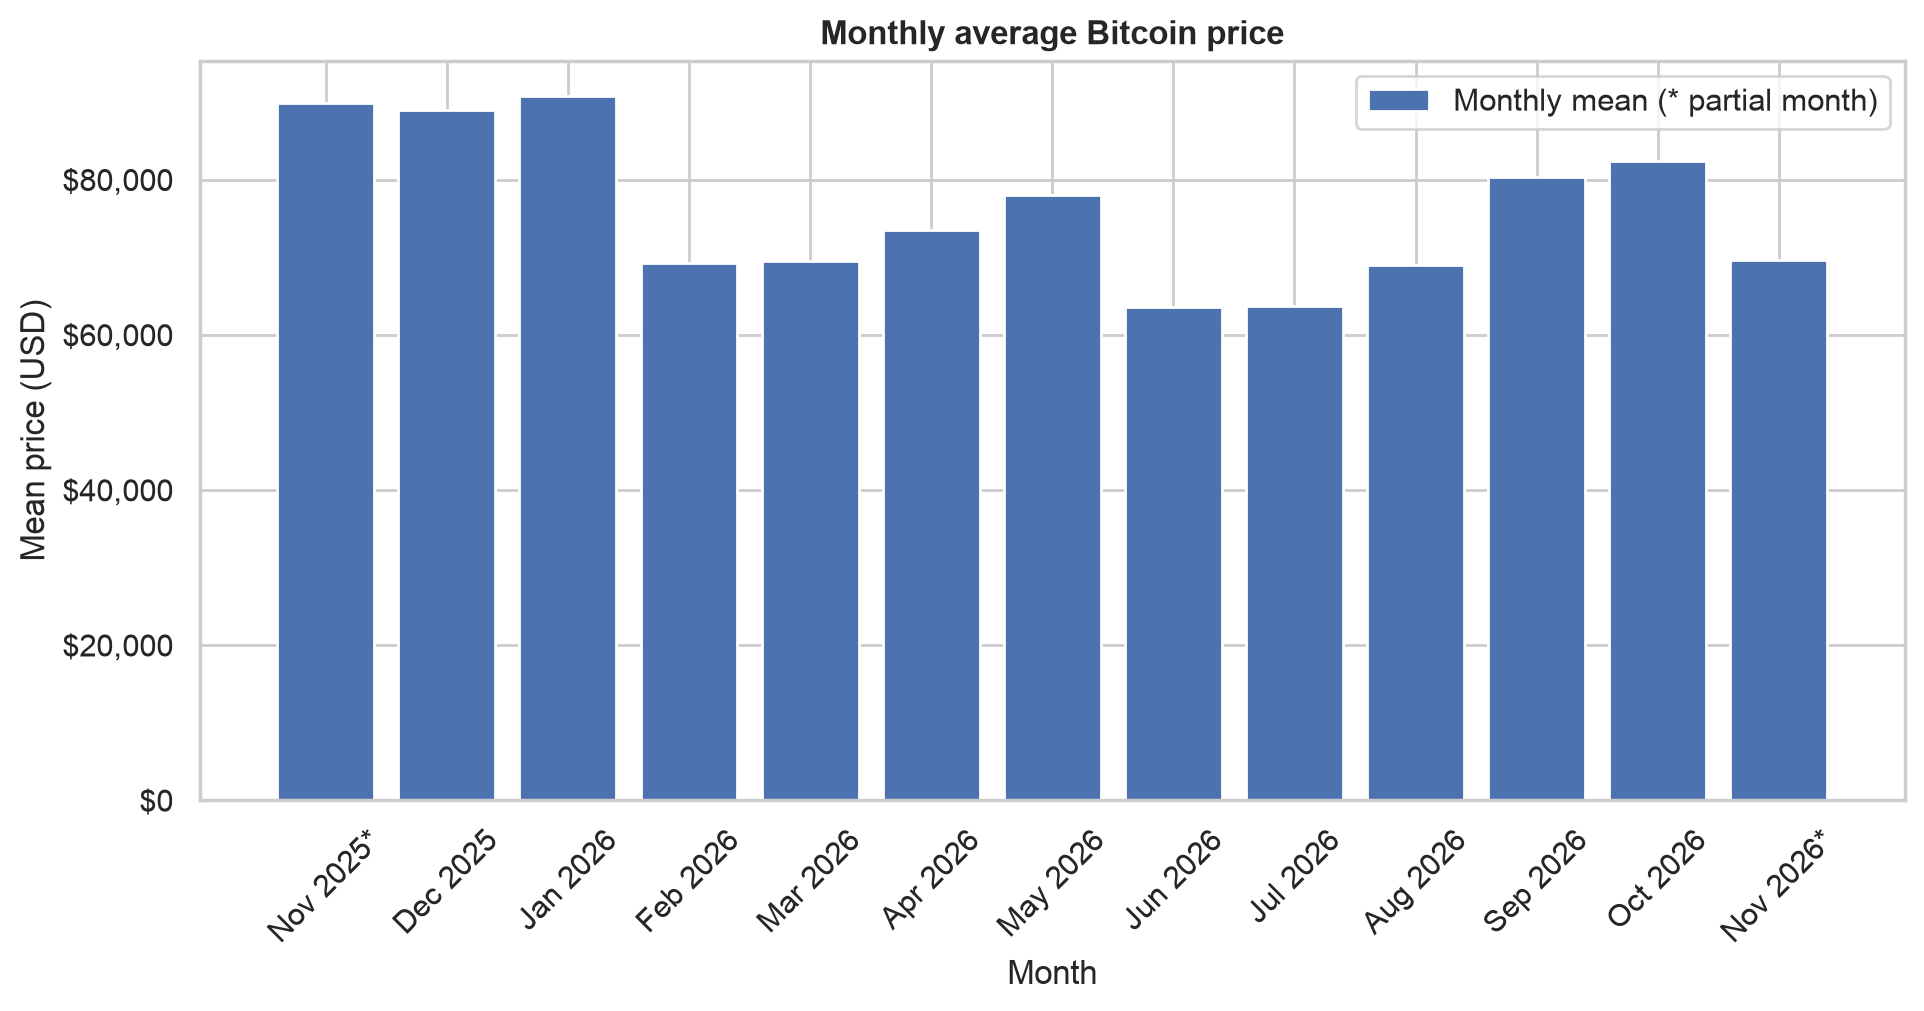
\includegraphics[width=\linewidth,height=0.78\textheight,keepaspectratio]{figures/monthly_average_price.png}
\caption{Monthly average price (asterisks mark partial months)}
\end{figure}

\begin{table}[H]
\centering
\caption{Monthly average price}
\small
\setlength{\tabcolsep}{4pt}
\begin{adjustbox}{max width=\linewidth}
\begin{tabular}{lrr}
\toprule
\textbf{Month} & \textbf{Mean price} & \textbf{Days} \\
\midrule
Nov 2025 & \$89,862.70 & 6 \\
Dec 2025 & \$89,010.16 & 31 \\
Jan 2026 & \$90,749.64 & 31 \\
Feb 2026 & \$69,229.64 & 28 \\
Mar 2026 & \$69,447.34 & 31 \\
Apr 2026 & \$73,476.72 & 30 \\
May 2026 & \$78,066.47 & 31 \\
Jun 2026 & \$63,502.69 & 30 \\
Jul 2026 & \$63,723.94 & 31 \\
Aug 2026 & \$68,978.17 & 31 \\
Sep 2026 & \$80,308.17 & 30 \\
Oct 2026 & \$82,326.52 & 31 \\
Nov 2026 & \$69,585.39 & 25 \\
\bottomrule
\end{tabular}
\end{adjustbox}
\end{table}

Monthly means were highest in January 2026 and lowest in June 2026. The first and last months are partial and are not directly comparable with full months.

\section{Stationarity Testing}

ARIMA assumes that the differenced series is stationary: its mean and autocovariance do not depend on time. Otherwise estimated relationships are unstable and can be spurious. Two complementary tests were used. The augmented Dickey-Fuller (ADF) test (Dickey and Fuller, 1979; Said and Dickey, 1984) estimates

\begin{equation}
\Delta y_t=\alpha+\beta t+\gamma y_{t-1}+\sum_{i=1}^{k}\delta_i\Delta y_{t-i}+\varepsilon_t
\end{equation}

ADF null hypothesis $H_0$: $\gamma = 0$ (unit root, non-stationary). Alternative $H_1$: $\gamma < 0$ (stationary around the included deterministic terms). Lag length k was chosen by AIC. The KPSS test (Kwiatkowski et al., 1992) reverses the hypotheses: $H_0$ is level (or trend) stationarity and $H_1$ is a unit root. The significance level was 5\%. KPSS p-values are interpolated from a table and truncated to the range 0.01 to 0.10.

\begin{table}[H]
\centering
\caption{ADF and KPSS results}
\footnotesize
\setlength{\tabcolsep}{4pt}
\begin{adjustbox}{max width=\linewidth}
\begin{tabular}{llllrrll}
\toprule
\textbf{Sample} & \textbf{Series} & \textbf{Test} & \textbf{Terms} & \textbf{Statistic} & \textbf{p} & \textbf{Critical 1/5/10\%} & \textbf{5\% result} \\
\midrule
Training & Price & ADF & constant & -1.757 & 0.402 & -3.453 / -2.872 / -2.572 & Non-stationary \\
Training & Price & KPSS & constant & 1.327 & $\le$0.010 & 0.739 / 0.463 / 0.347 & Non-stationary \\
Training & Price & ADF & constant + trend & -1.486 & 0.834 & -3.990 / -3.426 / -3.136 & Non-stationary \\
Training & Price & KPSS & constant + trend & 0.247 & $\le$0.010 & 0.216 / 0.146 / 0.119 & Non-stationary \\
Training & Log price & ADF & constant & -1.787 & 0.387 & -3.453 / -2.872 / -2.572 & Non-stationary \\
Training & Log price & KPSS & constant & 1.297 & $\le$0.010 & 0.739 / 0.463 / 0.347 & Non-stationary \\
Training & Log price & ADF & constant + trend & -1.529 & 0.819 & -3.990 / -3.426 / -3.136 & Non-stationary \\
Training & Log price & KPSS & constant + trend & 0.228 & $\le$0.010 & 0.216 / 0.146 / 0.119 & Non-stationary \\
Training & Differenced price & ADF & constant & -17.307 & \textless{}0.001 & -3.453 / -2.872 / -2.572 & Stationary \\
Training & Differenced price & KPSS & constant & 0.165 & $\ge$0.100 & 0.739 / 0.463 / 0.347 & Stationary \\
Training & Differenced log price & ADF & constant & -17.510 & \textless{}0.001 & -3.453 / -2.872 / -2.572 & Stationary \\
Training & Differenced log price & KPSS & constant & 0.162 & $\ge$0.100 & 0.739 / 0.463 / 0.347 & Stationary \\
Full & Price & ADF & constant & -1.570 & 0.499 & -3.448 / -2.869 / -2.571 & Non-stationary \\
Full & Price & KPSS & constant & 0.709 & 0.013 & 0.739 / 0.463 / 0.347 & Non-stationary \\
Full & Price & ADF & constant + trend & -1.725 & 0.740 & -3.984 / -3.423 / -3.134 & Non-stationary \\
Full & Price & KPSS & constant + trend & 0.384 & $\le$0.010 & 0.216 / 0.146 / 0.119 & Non-stationary \\
Full & Log price & ADF & constant & -2.047 & 0.267 & -3.449 / -2.870 / -2.571 & Non-stationary \\
Full & Log price & KPSS & constant & 0.672 & 0.016 & 0.739 / 0.463 / 0.347 & Non-stationary \\
Full & Log price & ADF & constant + trend & -2.245 & 0.465 & -3.984 / -3.423 / -3.134 & Non-stationary \\
Full & Log price & KPSS & constant + trend & 0.370 & $\le$0.010 & 0.216 / 0.146 / 0.119 & Non-stationary \\
Full & Differenced price & ADF & constant & -19.486 & \textless{}0.001 & -3.448 / -2.870 / -2.571 & Stationary \\
Full & Differenced price & KPSS & constant & 0.104 & $\ge$0.100 & 0.739 / 0.463 / 0.347 & Stationary \\
Full & Differenced log price & ADF & constant & -5.908 & \textless{}0.001 & -3.449 / -2.870 / -2.571 & Stationary \\
Full & Differenced log price & KPSS & constant & 0.108 & $\ge$0.100 & 0.739 / 0.463 / 0.347 & Stationary \\
\bottomrule
\end{tabular}
\end{adjustbox}
\end{table}

\begin{figure}[H]
\centering
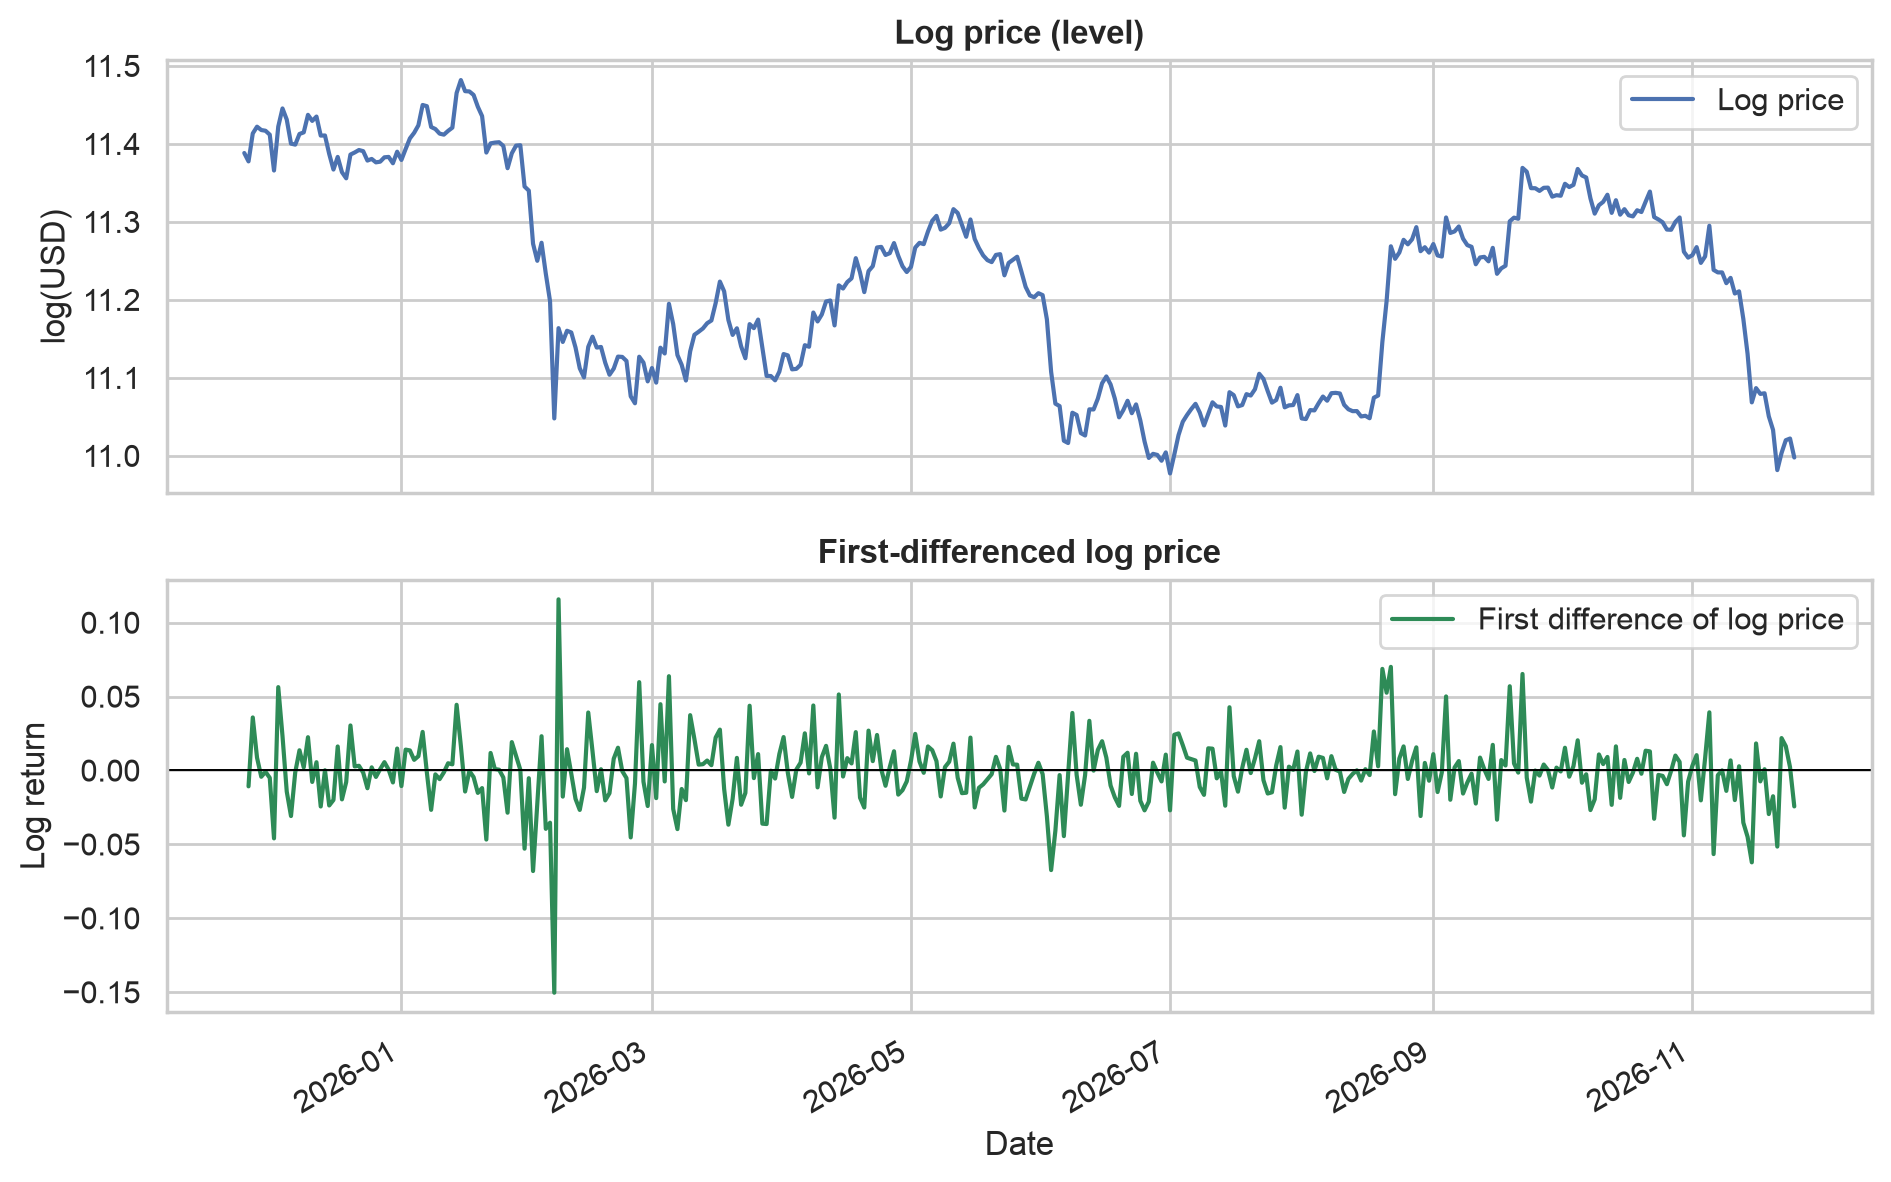
\includegraphics[width=\linewidth,height=0.78\textheight,keepaspectratio]{figures/differencing.png}
\caption{Log price before and after first differencing}
\end{figure}

For the training log price, ADF does not reject a unit root (statistic -1.787, p = 0.387) and KPSS rejects stationarity. After one difference ADF rejects the unit root (statistic -17.510, p \textless{} 0.001) and KPSS does not reject stationarity. The full sample agrees. The smallest order that passes is therefore d = 1; further differencing was not applied, as it would risk over-differencing. The order was determined on training data only. Mean stationarity does not imply constant variance, which is examined in the residual diagnostics.

\section{ACF and PACF Analysis}

The autocorrelation function (ACF) measures correlation between a series and its lag k. The partial autocorrelation function (PACF) measures that correlation after removing intermediate lags. In textbook cases a pure AR(p) process has a PACF that cuts off after lag p, and a pure MA(q) process has an ACF that cuts off after lag q.

\begin{figure}[H]
\centering
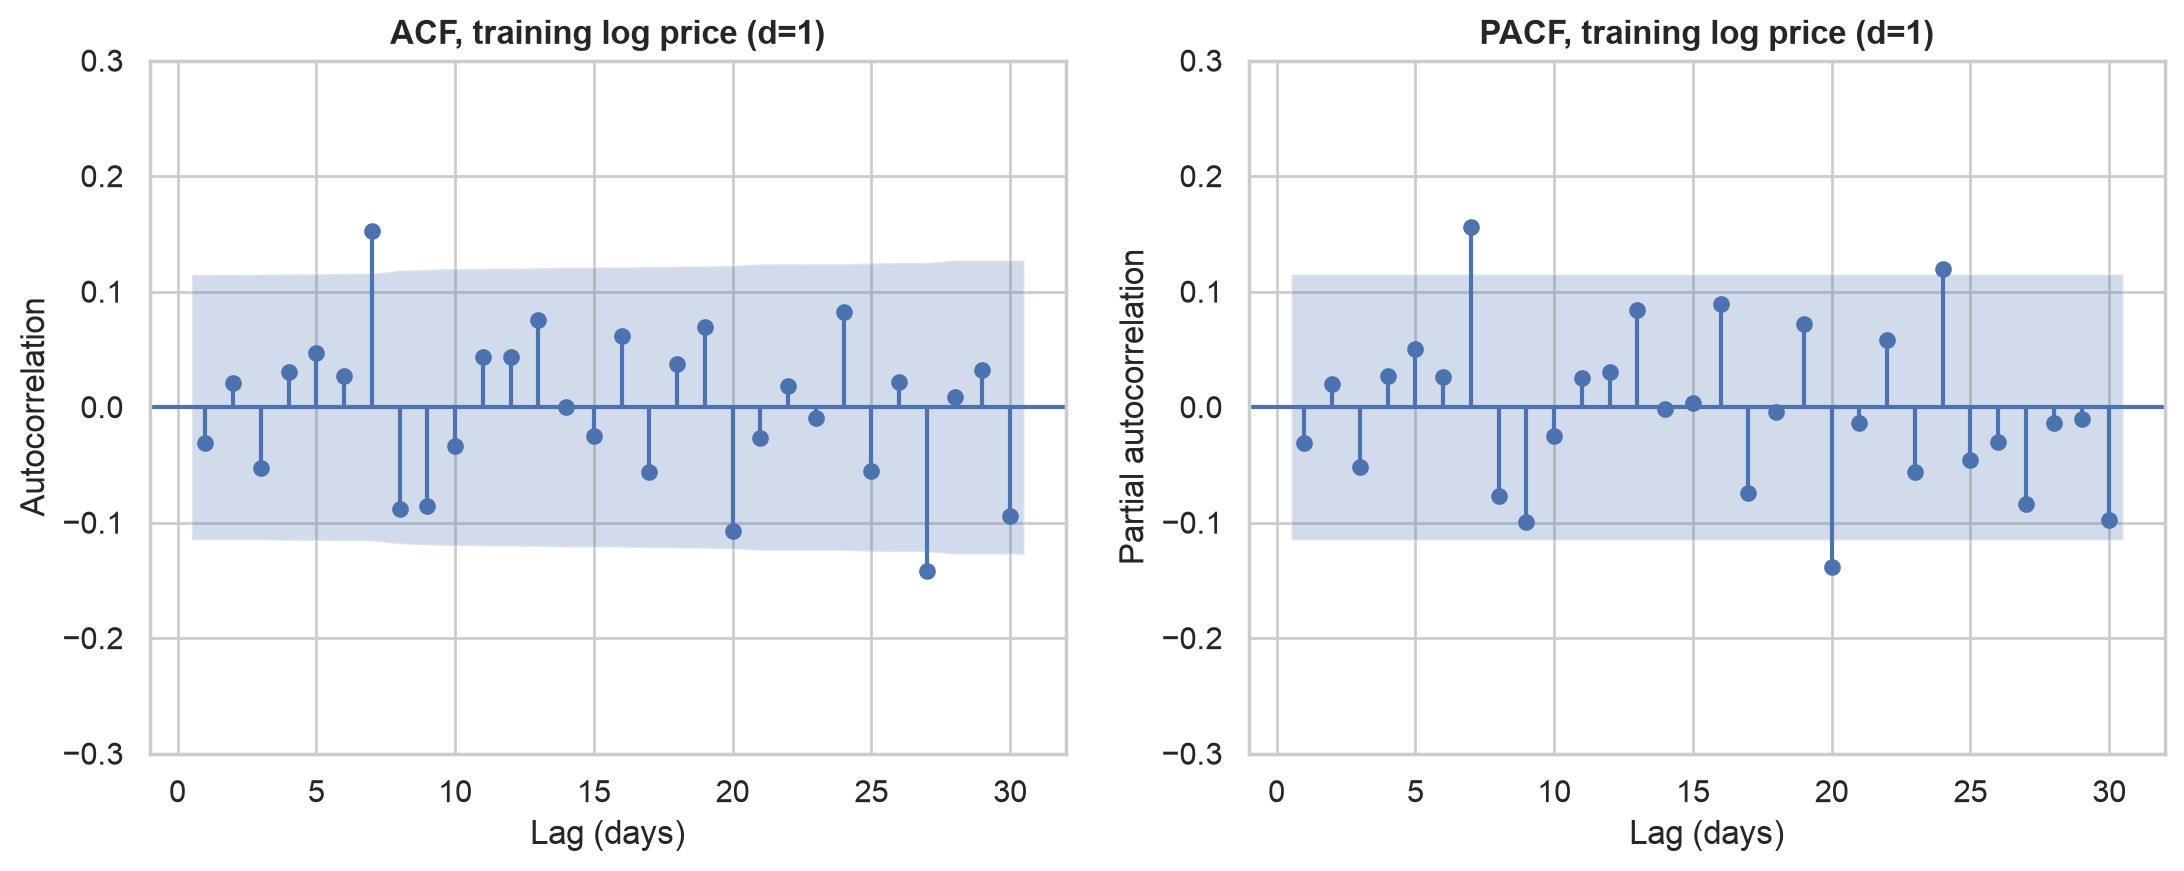
\includegraphics[width=\linewidth,height=0.78\textheight,keepaspectratio]{figures/acf_pacf.png}
\caption{ACF and PACF of the differenced training log price}
\end{figure}

With n = 291, the approximate 95\% bound is $\pm$0.115. ACF values outside it: lag 7 (0.152), lag 27 (-0.142). PACF values outside it: lag 7 (0.156), lag 20 (-0.138), lag 24 (0.119). Lags 1 to 6 are all insignificant, which points to little short-term linear dependence and is consistent with p = q = 0. The lag-7 spike could reflect a weekly effect, so the grid was extended to p, q $\le$ 7.

These plots have clear limits. With 30 lags, about one or two spikes would be expected outside 95\% bounds by chance. The bounds assume independent, constant-variance noise, which is doubtful here. Mixed ARMA processes produce no clean cut-off. The plots therefore guided the search range but did not choose the model.

\section{ARIMA Model Development}

All combinations of p = 0 to 7, d = 1 and q = 0 to 7, with and without drift, were estimated on the training sample (128 models; 121 converged). Fit was compared by the Akaike (1974) and Schwarz (1978) criteria, where k is the number of parameters, n the sample size and L the maximised likelihood:

\begin{equation}
AIC=2k-2\ln\hat L,\qquad BIC=k\ln n-2\ln\hat L
\end{equation}

\begin{table}[H]
\centering
\caption{Five best grid models by AIC and by BIC (training sample)}
\footnotesize
\setlength{\tabcolsep}{4pt}
\begin{adjustbox}{max width=\linewidth}
\begin{tabular}{llrrrl}
\toprule
\textbf{Ranking} & \textbf{Model} & \textbf{AIC} & \textbf{BIC} & \textbf{Min. root} & \textbf{Converged} \\
\midrule
AIC & ARIMA(6, 1, 5) & -1361.30 & -1317.22 & 1.00004 & True \\
AIC & ARIMA(4, 1, 4) & -1360.82 & -1327.76 & 1.00001 & True \\
AIC & ARIMA(4, 1, 5) & -1359.94 & -1323.20 & 1.00000 & True \\
AIC & ARIMA(6, 1, 4) & -1359.24 & -1318.83 & 1.00000 & True \\
AIC & ARIMA(3, 1, 2) & -1358.89 & -1336.85 & 1.00118 & True \\
BIC & ARIMA(0, 1, 0) & -1351.45 & -1347.77 & none & True \\
BIC & ARIMA(1, 1, 0) & -1349.72 & -1342.37 & 32.46591 & False \\
BIC & ARIMA(0, 1, 1) & -1349.71 & -1342.36 & 34.55656 & True \\
BIC & ARIMA(0, 1, 0) + drift & -1349.56 & -1342.21 & none & True \\
BIC & ARIMA(1, 1, 1) & -1348.04 & -1337.02 & 1.79514 & True \\
\bottomrule
\end{tabular}
\end{adjustbox}
\end{table}

The criteria disagree. AIC prefers large models such as ARIMA(6, 1, 5), while BIC, which penalises complexity more heavily, prefers ARIMA(0, 1, 0). A stepwise pmdarima auto\_arima search also returned ARIMA(0, 1, 0); it follows the automatic-search idea of Hyndman and Khandakar (2008) and was treated as one candidate rather than an authority.

\subsection{Selection rule}

\begin{enumerate}
  \item Shortlist the five best AIC models, the five best BIC models, the auto\_arima result and the random walk.
  \item Reject models that did not converge or fail the Ljung-Box test at 5\% (lags 10, 20, where the lag exceeds p + q).
  \item Reject models with any AR or MA root of modulus below 1.001.
  \item Among the rest, take the lowest seven-day rolling-origin RMSE over the last 58 training observations (from 2026-07-17); within 1\% of the best, take the fewest parameters.
\end{enumerate}

\begin{table}[H]
\centering
\caption{Shortlisted models: diagnostics and validation accuracy (Params includes the error variance)}
\footnotesize
\setlength{\tabcolsep}{4pt}
\begin{adjustbox}{max width=\linewidth}
\begin{tabular}{lrrllrr}
\toprule
\textbf{Model} & \textbf{Params} & \textbf{LB min p} & \textbf{Converged} & \textbf{Roots admissible} & \textbf{Val. RMSE 1-day} & \textbf{Val. RMSE 7-day} \\
\midrule
ARIMA(6, 1, 4) & 11 & 0.173 & True & False & 1,479 & 3,679 \\
ARIMA(6, 1, 5) & 12 & 0.360 & True & False & 1,505 & 3,721 \\
ARIMA(0, 1, 0) & 1 & 0.163 & True & True & 1,444 & 3,742 \\
ARIMA(4, 1, 4) & 9 & 0.010 & True & False & 1,521 & 3,747 \\
ARIMA(4, 1, 5) & 10 & 0.023 & True & False & 1,438 & 3,747 \\
ARIMA(3, 1, 2) & 6 & 0.066 & True & True & 1,446 & 3,751 \\
ARIMA(1, 1, 0) & 2 & 0.121 & False & True & 1,463 & 3,760 \\
ARIMA(0, 1, 1) & 2 & 0.122 & True & True & 1,464 & 3,762 \\
ARIMA(1, 1, 1) & 3 & 0.083 & True & True & 1,471 & 3,775 \\
ARIMA(0, 1, 0) + drift & 2 & 0.163 & True & True & 1,457 & 3,863 \\
\bottomrule
\end{tabular}
\end{adjustbox}
\end{table}

\subsection{A disclosed revision to the rule}

The first run of this analysis did not include the root screen and selected ARIMA(6, 1, 4), whose seven-day validation RMSE (3,679) was 1.7\% below that of ARIMA(0, 1, 0) (3,742). Inspection showed that its smallest MA root modulus was 1.000004, essentially on the unit circle. This indicates a non-invertible, probably over-parameterised fit: moving-average standard errors were extremely large in the training fit, and on the full sample its residuals failed Ljung-Box at lag 20 (p = 0.046). The threshold of 1.001 follows Hyndman and Khandakar (2008). The screen itself uses only training-sample estimates, but it was added after the first results, including test results, had been seen. The selection is therefore not fully blind. To show the effect of this decision, ARIMA(6, 1, 4) is retained throughout as a sensitivity analysis.

The final specification is ARIMA(0, 1, 0):

\begin{equation}
y_t=y_{t-1}+\varepsilon_t,\qquad \hat y_{T+h}=y_T,\qquad \sigma_h^2=h\,\sigma^2
\end{equation}

It has one estimated parameter, the error variance (full-sample estimate 0.000543, standard error 0.000020, equivalent to a daily log-price standard deviation of 2.33\%). It is appropriate here because it has the lowest BIC, agrees with auto\_arima, passes the pre-set diagnostic screen and has the lowest validation RMSE among admissible candidates. `Appropriate' means that the data do not justify a more complex linear mean model; it does not mean the model describes all features of the series.

\section{Training and Testing}

The split was chronological: training 2025-11-25 to 2026-09-12 (n = 292, 80\%) and testing 2026-09-13 to 2026-11-25 (n = 74, 20\%). Random shuffling would let a model learn from observations later than those it predicts and would destroy the lag structure, a form of data leakage that overstates accuracy. Three test designs were used (Tashman, 2000):

\begin{itemize}
  \item One-step walk-forward: refit on all data up to each day and predict the next day.
  \item Seven-day rolling origin: refit at 68 successive origins and predict one to seven days ahead (476 overlapping forecasts), matching the assignment horizon.
  \item Static multi-step: one fit on the training set forecasting all 74 test days.
\end{itemize}

The model order stayed fixed during testing; only parameters were re-estimated. The optimiser reported a convergence warning at 5 one-step origins. For the random walk the point forecast is the last observation regardless of the variance estimate, so this does not affect point accuracy.

\section{Model Evaluation}

For actual values A(t), forecasts F(t) and n forecasts:

\begin{equation}
MAE=\frac{1}{n}\sum|A_t-F_t|,\qquad RMSE=\sqrt{\frac{1}{n}\sum(A_t-F_t)^2}
\end{equation}

\begin{equation}
\begin{gathered}
MAPE=\frac{100}{n}\sum\frac{|A_t-F_t|}{|A_t|},\\ sMAPE=\frac{100}{n}\sum\frac{2|A_t-F_t|}{|A_t|+|F_t|}
\end{gathered}
\end{equation}

\begin{equation}
DA=\frac{100}{m}\sum 1[\,\mathrm{sign}(F_t-P_o)=\mathrm{sign}(A_t-P_o)\,]
\end{equation}

P(o) is the price at the forecast origin and m counts forecasts that state a direction. MAE is the typical dollar error. RMSE penalises large errors more. MAPE and sMAPE express errors relative to price. MAPE is stable here because prices are far from zero (Hyndman and Koehler, 2006 discuss its weaknesses), but a low MAPE on price levels mostly reflects the fact that tomorrow's price is close to today's. It is not evidence of skill. Directional accuracy is undefined for a forecast of no change.

\begin{table}[H]
\centering
\caption{Test accuracy of the selected model and baselines}
\footnotesize
\setlength{\tabcolsep}{4pt}
\begin{adjustbox}{max width=\linewidth}
\begin{tabular}{llrrrrrl}
\toprule
\textbf{Evaluation} & \textbf{Model} & \textbf{n} & \textbf{MAE} & \textbf{RMSE} & \textbf{MAPE \%} & \textbf{sMAPE \%} & \textbf{Dir. acc. \%} \\
\midrule
1-step walk-forward & ARIMA(0, 1, 0) & 74 & 1,141 & 1,651 & 1.51 & 1.50 & n/a \\
1-step walk-forward & Naive (last value) & 74 & 1,141 & 1,651 & 1.51 & 1.50 & n/a \\
1-step walk-forward & Drift & 74 & 1,142 & 1,647 & 1.51 & 1.50 & 52.7 \\
1-step walk-forward & 7-day moving average & 74 & 2,142 & 2,851 & 2.90 & 2.86 & 60.8 \\
7-day rolling origin & ARIMA(0, 1, 0) & 476 & 2,458 & 3,445 & 3.29 & 3.24 & n/a \\
7-day rolling origin & Naive (last value) & 476 & 2,458 & 3,445 & 3.29 & 3.24 & n/a \\
7-day rolling origin & Drift & 476 & 2,420 & 3,406 & 3.23 & 3.18 & 65.5 \\
7-day rolling origin & 7-day moving average & 476 & 3,311 & 4,479 & 4.52 & 4.39 & 47.5 \\
Static multi-step & ARIMA(0, 1, 0) & 74 & 5,968 & 7,512 & 8.17 & 7.90 & n/a \\
Static multi-step & Naive (last value) & 74 & 5,968 & 7,512 & 8.17 & 7.90 & n/a \\
\bottomrule
\end{tabular}
\end{adjustbox}
\end{table}

\begin{figure}[H]
\centering
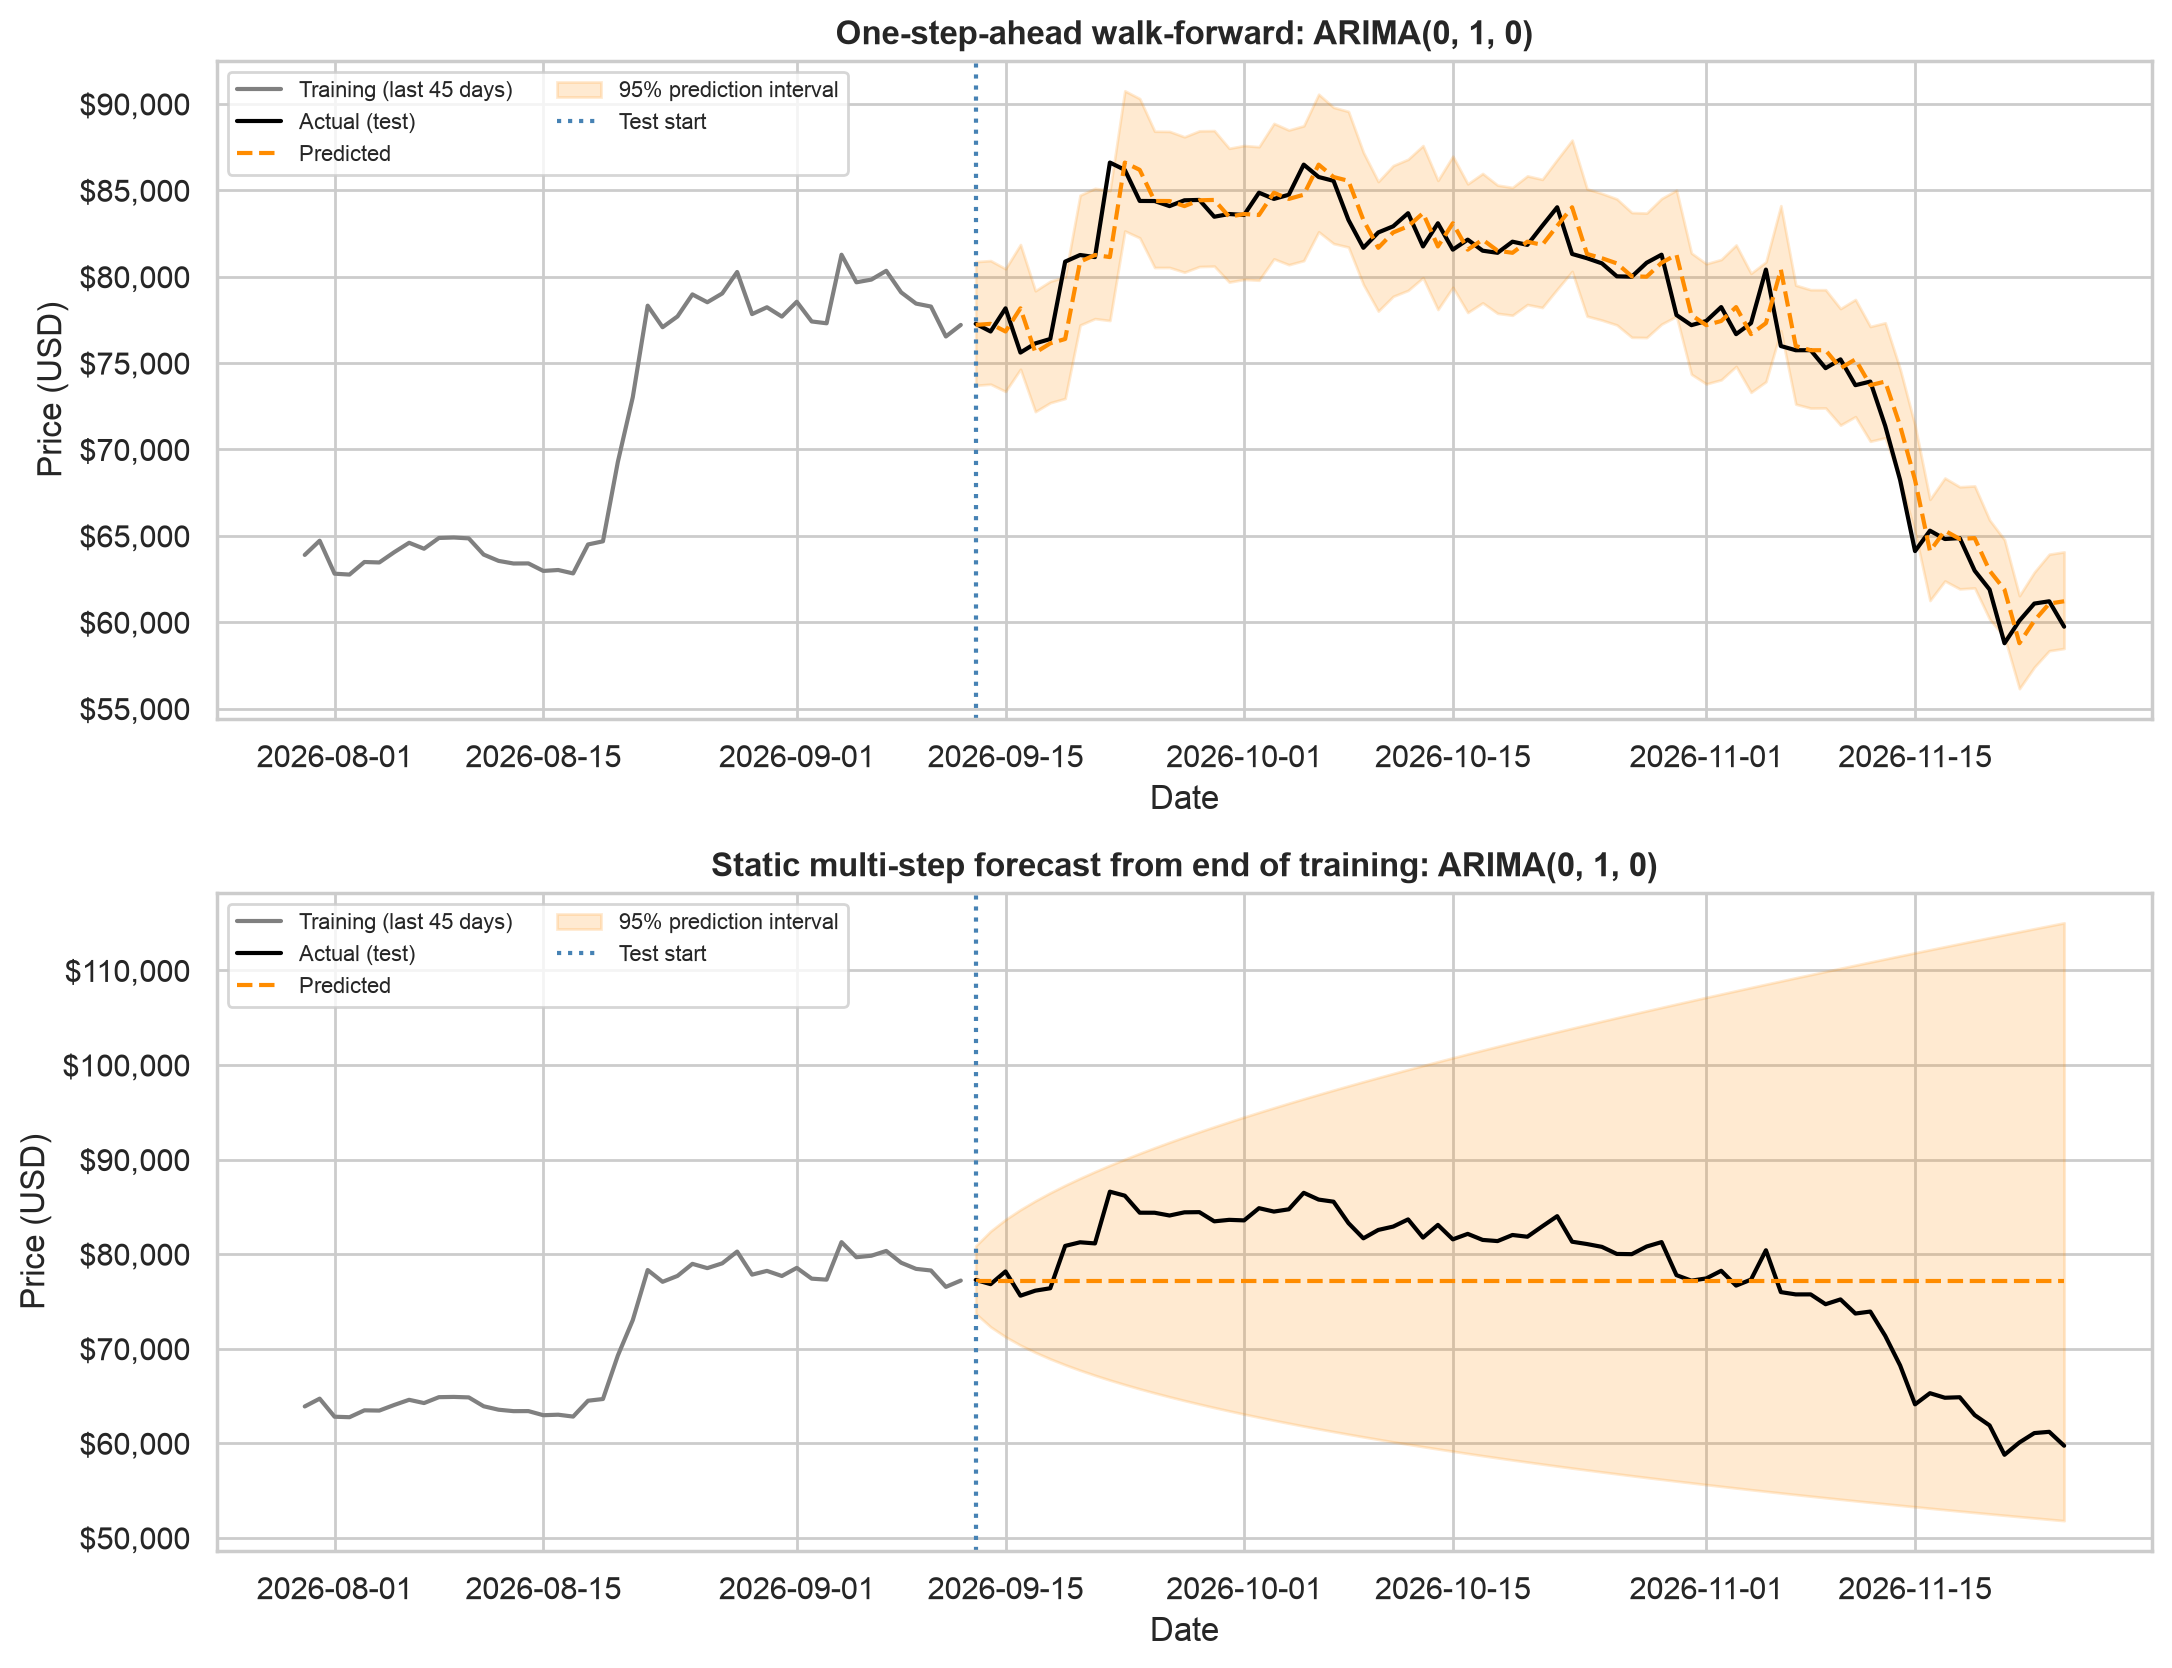
\includegraphics[width=\linewidth,height=0.78\textheight,keepaspectratio]{figures/test_predictions.png}
\caption{Test-period forecasts and 95\% prediction intervals}
\end{figure}

The selected model and the naive baseline are identical, so their errors match exactly. The drift baseline had slightly lower RMSE (one-step 1,647 against 1,651; seven-day 3,406 against 3,445). The test period ended in a strong decline, and 39 of 74 one-day moves were downward; a persistently negative drift benefits from such a period, so its directional score is not evidence of general forecasting ability. The seven-day moving average was clearly worst on error size.

In the one-step plot the forecast is the actual series shifted by one day. The visual closeness must not be mistaken for prediction. The static forecast (MAPE 8.17\%) shows how quickly information decays: it remains at the last training price while the market rises and then falls.

Empirical coverage of the nominal 95\% interval was 93.2\% one day ahead and 88.2\% seven days ahead. The forecasts overlap and the sample is short, but the seven-day intervals appear somewhat too narrow. Static coverage of 100\% comes from a single forecast path and is not informative.

\begin{table}[H]
\centering
\caption{Actual and predicted prices, first ten test days (all days in the Appendix)}
\small
\setlength{\tabcolsep}{4pt}
\begin{adjustbox}{max width=\linewidth}
\begin{tabular}{rrrrr}
\toprule
\textbf{Date} & \textbf{Actual} & \textbf{Predicted} & \textbf{Absolute error} & \textbf{Percentage error} \\
\midrule
2026-09-13 & \$77,273.07 & \$77,209.87 & \$63.20 & 0.08\% \\
2026-09-14 & \$76,829.51 & \$77,273.07 & \$443.56 & 0.58\% \\
2026-09-15 & \$78,169.72 & \$76,829.51 & \$1,340.21 & 1.71\% \\
2026-09-16 & \$75,609.19 & \$78,169.72 & \$2,560.53 & 3.39\% \\
2026-09-17 & \$76,141.53 & \$75,609.19 & \$532.34 & 0.70\% \\
2026-09-18 & \$76,395.02 & \$76,141.53 & \$253.49 & 0.33\% \\
2026-09-19 & \$80,872.23 & \$76,395.02 & \$4,477.21 & 5.54\% \\
2026-09-20 & \$81,256.73 & \$80,872.23 & \$384.50 & 0.47\% \\
2026-09-21 & \$81,136.20 & \$81,256.73 & \$120.53 & 0.15\% \\
2026-09-22 & \$86,607.63 & \$81,136.20 & \$5,471.43 & 6.32\% \\
\bottomrule
\end{tabular}
\end{adjustbox}
\end{table}

\subsection{Comparison with other candidates (post-hoc)}

\begin{table}[H]
\centering
\caption{Test accuracy of the other shortlisted models (not used for selection)}
\footnotesize
\setlength{\tabcolsep}{4pt}
\begin{adjustbox}{max width=\linewidth}
\begin{tabular}{llrrrrrr}
\toprule
\textbf{Evaluation} & \textbf{Model} & \textbf{n} & \textbf{MAE} & \textbf{RMSE} & \textbf{MAPE \%} & \textbf{sMAPE \%} & \textbf{Dir. acc. \%} \\
\midrule
1-step walk-forward & ARIMA(6, 1, 4) & 74 & 1,172 & 1,651 & 1.54 & 1.54 & 56.8 \\
7-day rolling origin & ARIMA(6, 1, 4) & 476 & 2,390 & 3,343 & 3.18 & 3.13 & 58.6 \\
1-step walk-forward & ARIMA(6, 1, 5) & 74 & 1,191 & 1,671 & 1.57 & 1.57 & 58.1 \\
7-day rolling origin & ARIMA(6, 1, 5) & 476 & 2,382 & 3,347 & 3.18 & 3.12 & 59.2 \\
1-step walk-forward & ARIMA(4, 1, 4) & 74 & 1,119 & 1,614 & 1.49 & 1.48 & 63.5 \\
7-day rolling origin & ARIMA(4, 1, 4) & 476 & 2,391 & 3,354 & 3.19 & 3.14 & 59.2 \\
1-step walk-forward & ARIMA(4, 1, 5) & 74 & 1,163 & 1,604 & 1.53 & 1.52 & 59.5 \\
7-day rolling origin & ARIMA(4, 1, 5) & 476 & 2,349 & 3,297 & 3.14 & 3.08 & 61.8 \\
1-step walk-forward & ARIMA(3, 1, 2) & 74 & 1,156 & 1,637 & 1.53 & 1.52 & 59.5 \\
7-day rolling origin & ARIMA(3, 1, 2) & 476 & 2,476 & 3,466 & 3.32 & 3.26 & 46.2 \\
1-step walk-forward & ARIMA(1, 1, 0) & 74 & 1,142 & 1,652 & 1.51 & 1.50 & 58.1 \\
7-day rolling origin & ARIMA(1, 1, 0) & 476 & 2,461 & 3,450 & 3.30 & 3.24 & 52.7 \\
1-step walk-forward & ARIMA(0, 1, 1) & 74 & 1,142 & 1,652 & 1.51 & 1.50 & 56.8 \\
7-day rolling origin & ARIMA(0, 1, 1) & 476 & 2,462 & 3,451 & 3.30 & 3.24 & 51.3 \\
1-step walk-forward & ARIMA(1, 1, 1) & 74 & 1,144 & 1,654 & 1.51 & 1.51 & 47.3 \\
7-day rolling origin & ARIMA(1, 1, 1) & 476 & 2,462 & 3,451 & 3.30 & 3.24 & 44.3 \\
1-step walk-forward & ARIMA(0, 1, 0) + drift & 74 & 1,142 & 1,647 & 1.51 & 1.50 & 52.7 \\
7-day rolling origin & ARIMA(0, 1, 0) + drift & 476 & 2,419 & 3,405 & 3.23 & 3.18 & 65.5 \\
\bottomrule
\end{tabular}
\end{adjustbox}
\end{table}

Some more complex models, notably ARIMA(4, 1, 4) and ARIMA(4, 1, 5), had lower test errors than the random walk. Both failed the pre-set screen, and choosing them now would be selection on the test set. Diebold-Mariano tests on one-step squared errors with the small-sample correction (Diebold and Mariano, 1995; Harvey et al., 1997) found no model significantly different from the naive forecast (smallest p = 0.160). For ARIMA(6, 1, 4), p = 0.987.

\section{Residual Diagnostics}

An adequate mean model should leave residuals resembling white noise. The Ljung and Box (1978) statistic, with $H_0$ of no autocorrelation up to lag h, is

\begin{equation}
Q=n(n+2)\sum_{k=1}^{h}\frac{\hat\rho_k^2}{n-k}\ \sim\ \chi^2_{h-p-q}
\end{equation}

\begin{figure}[H]
\centering
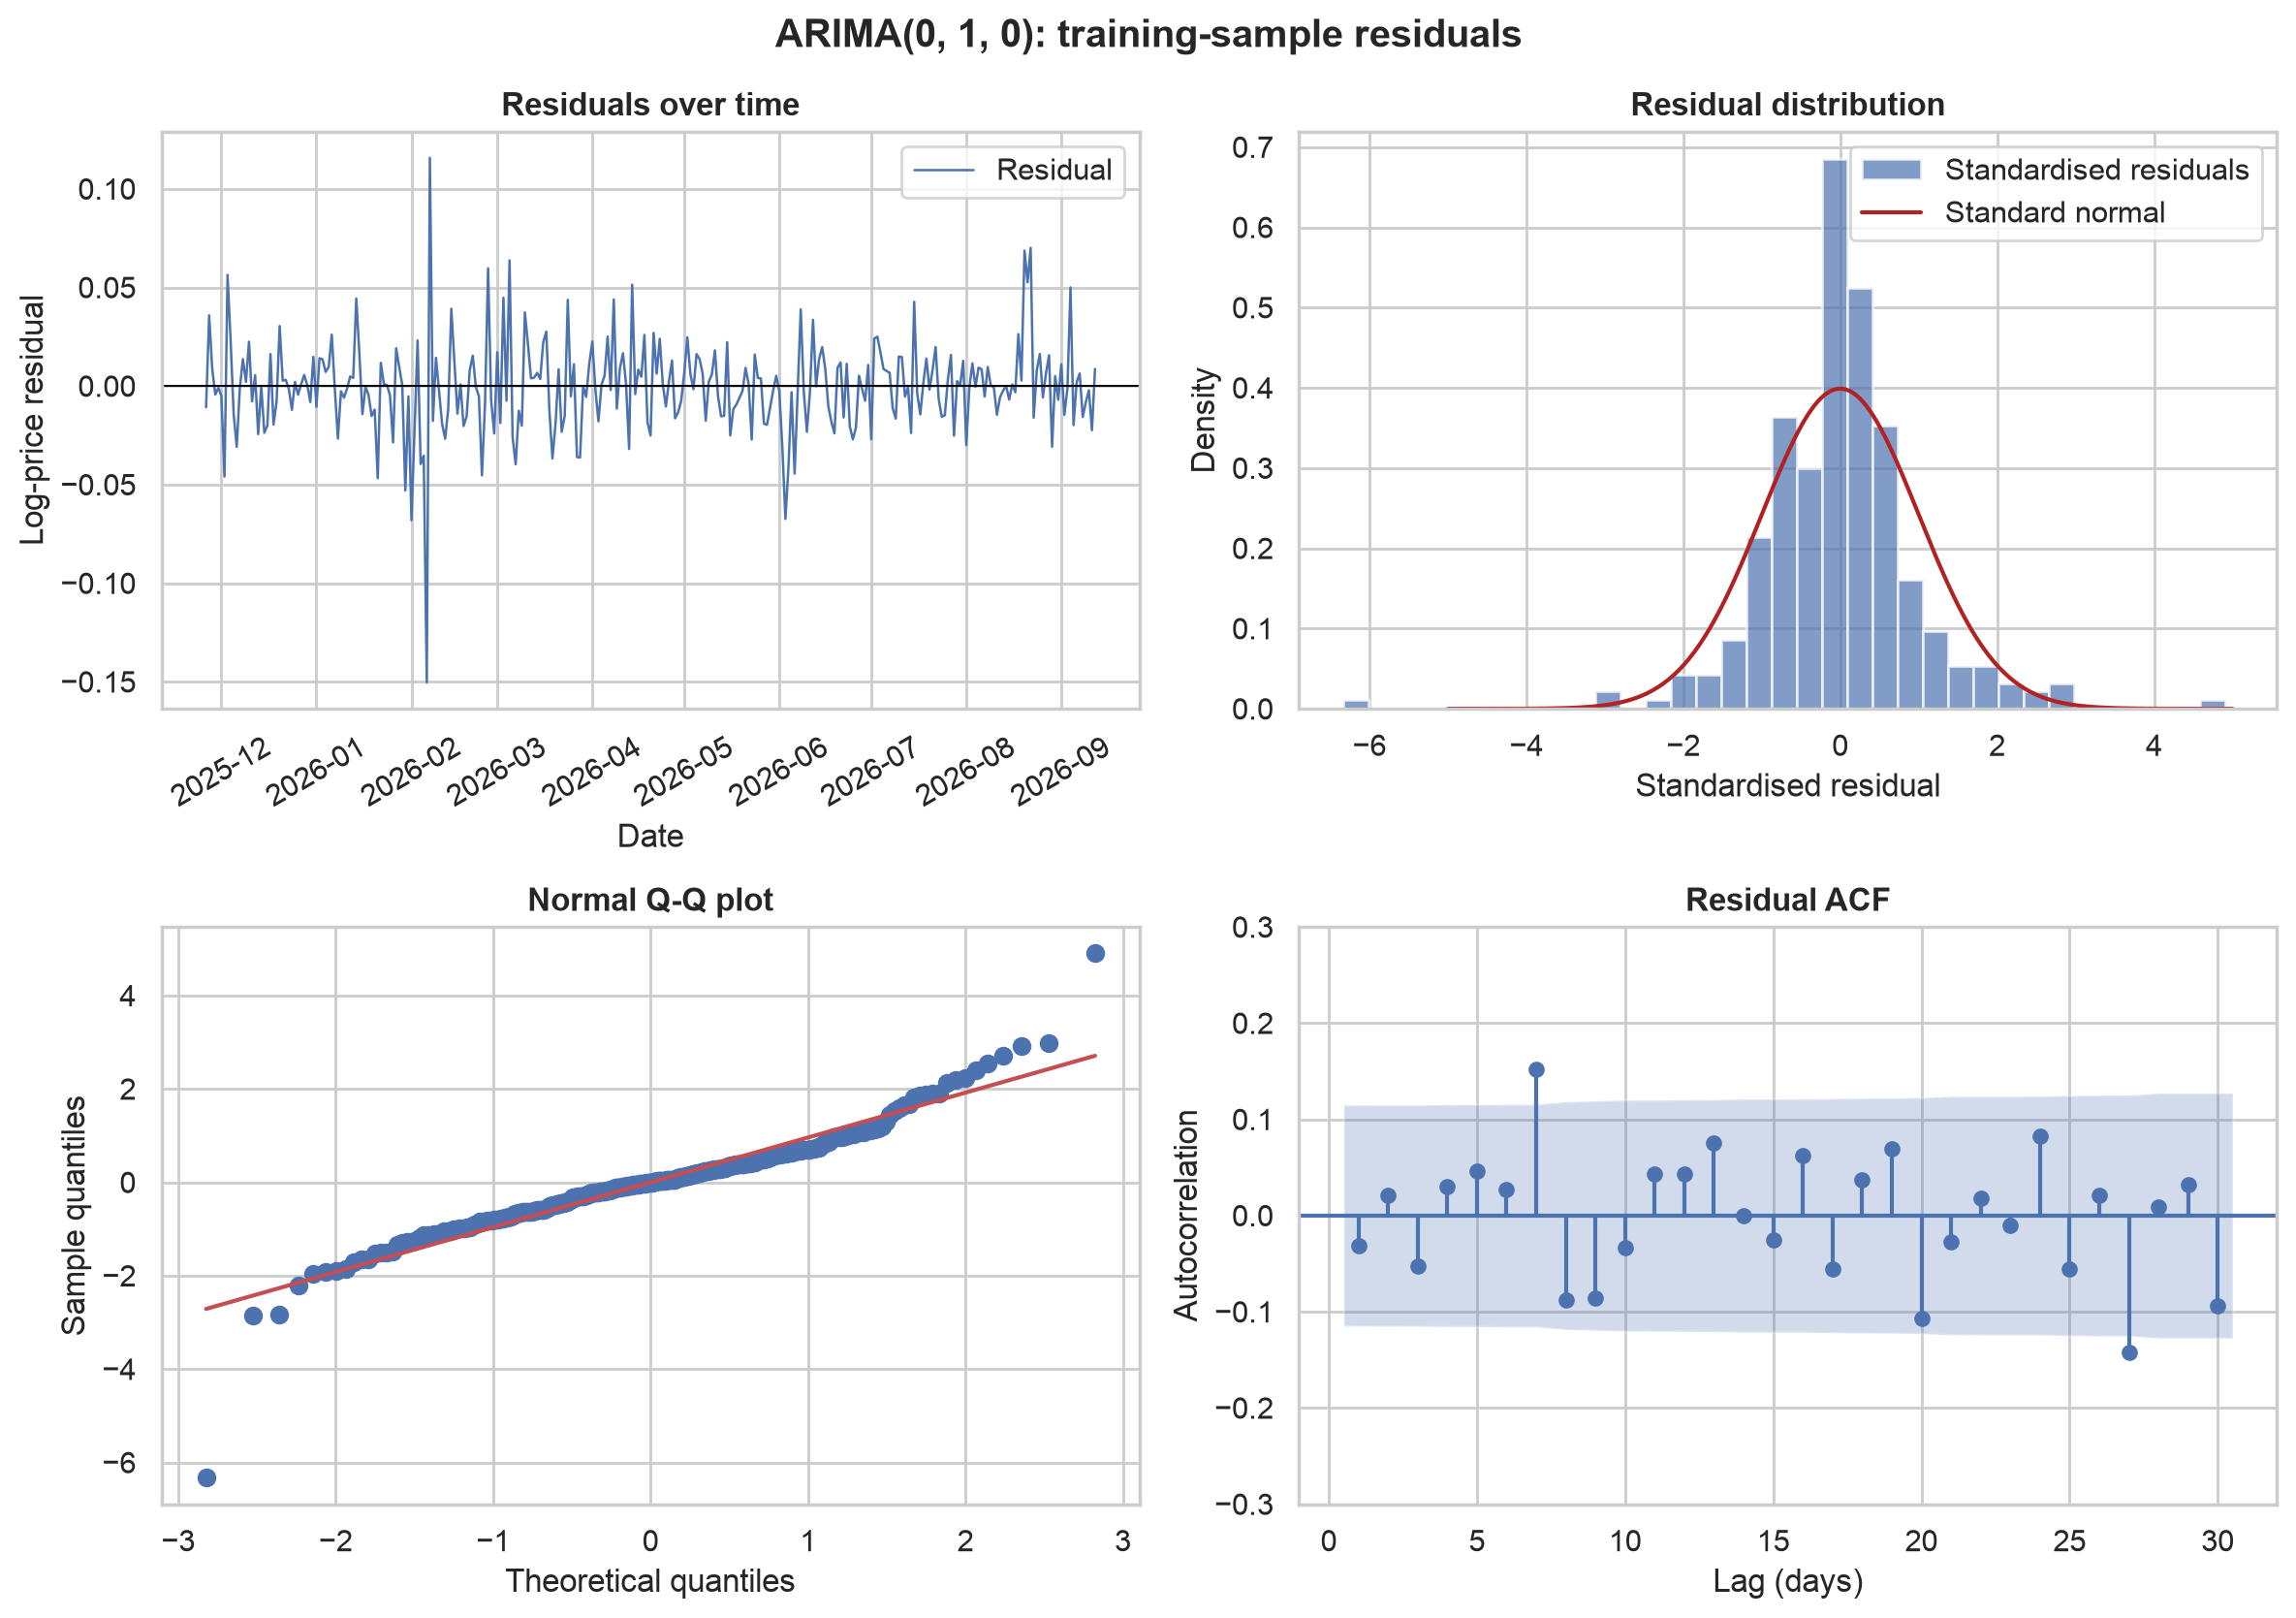
\includegraphics[width=\linewidth,height=0.78\textheight,keepaspectratio]{figures/model_diagnostics.png}
\caption{Residual diagnostics, ARIMA(0, 1, 0), training sample}
\end{figure}

\begin{figure}[H]
\centering
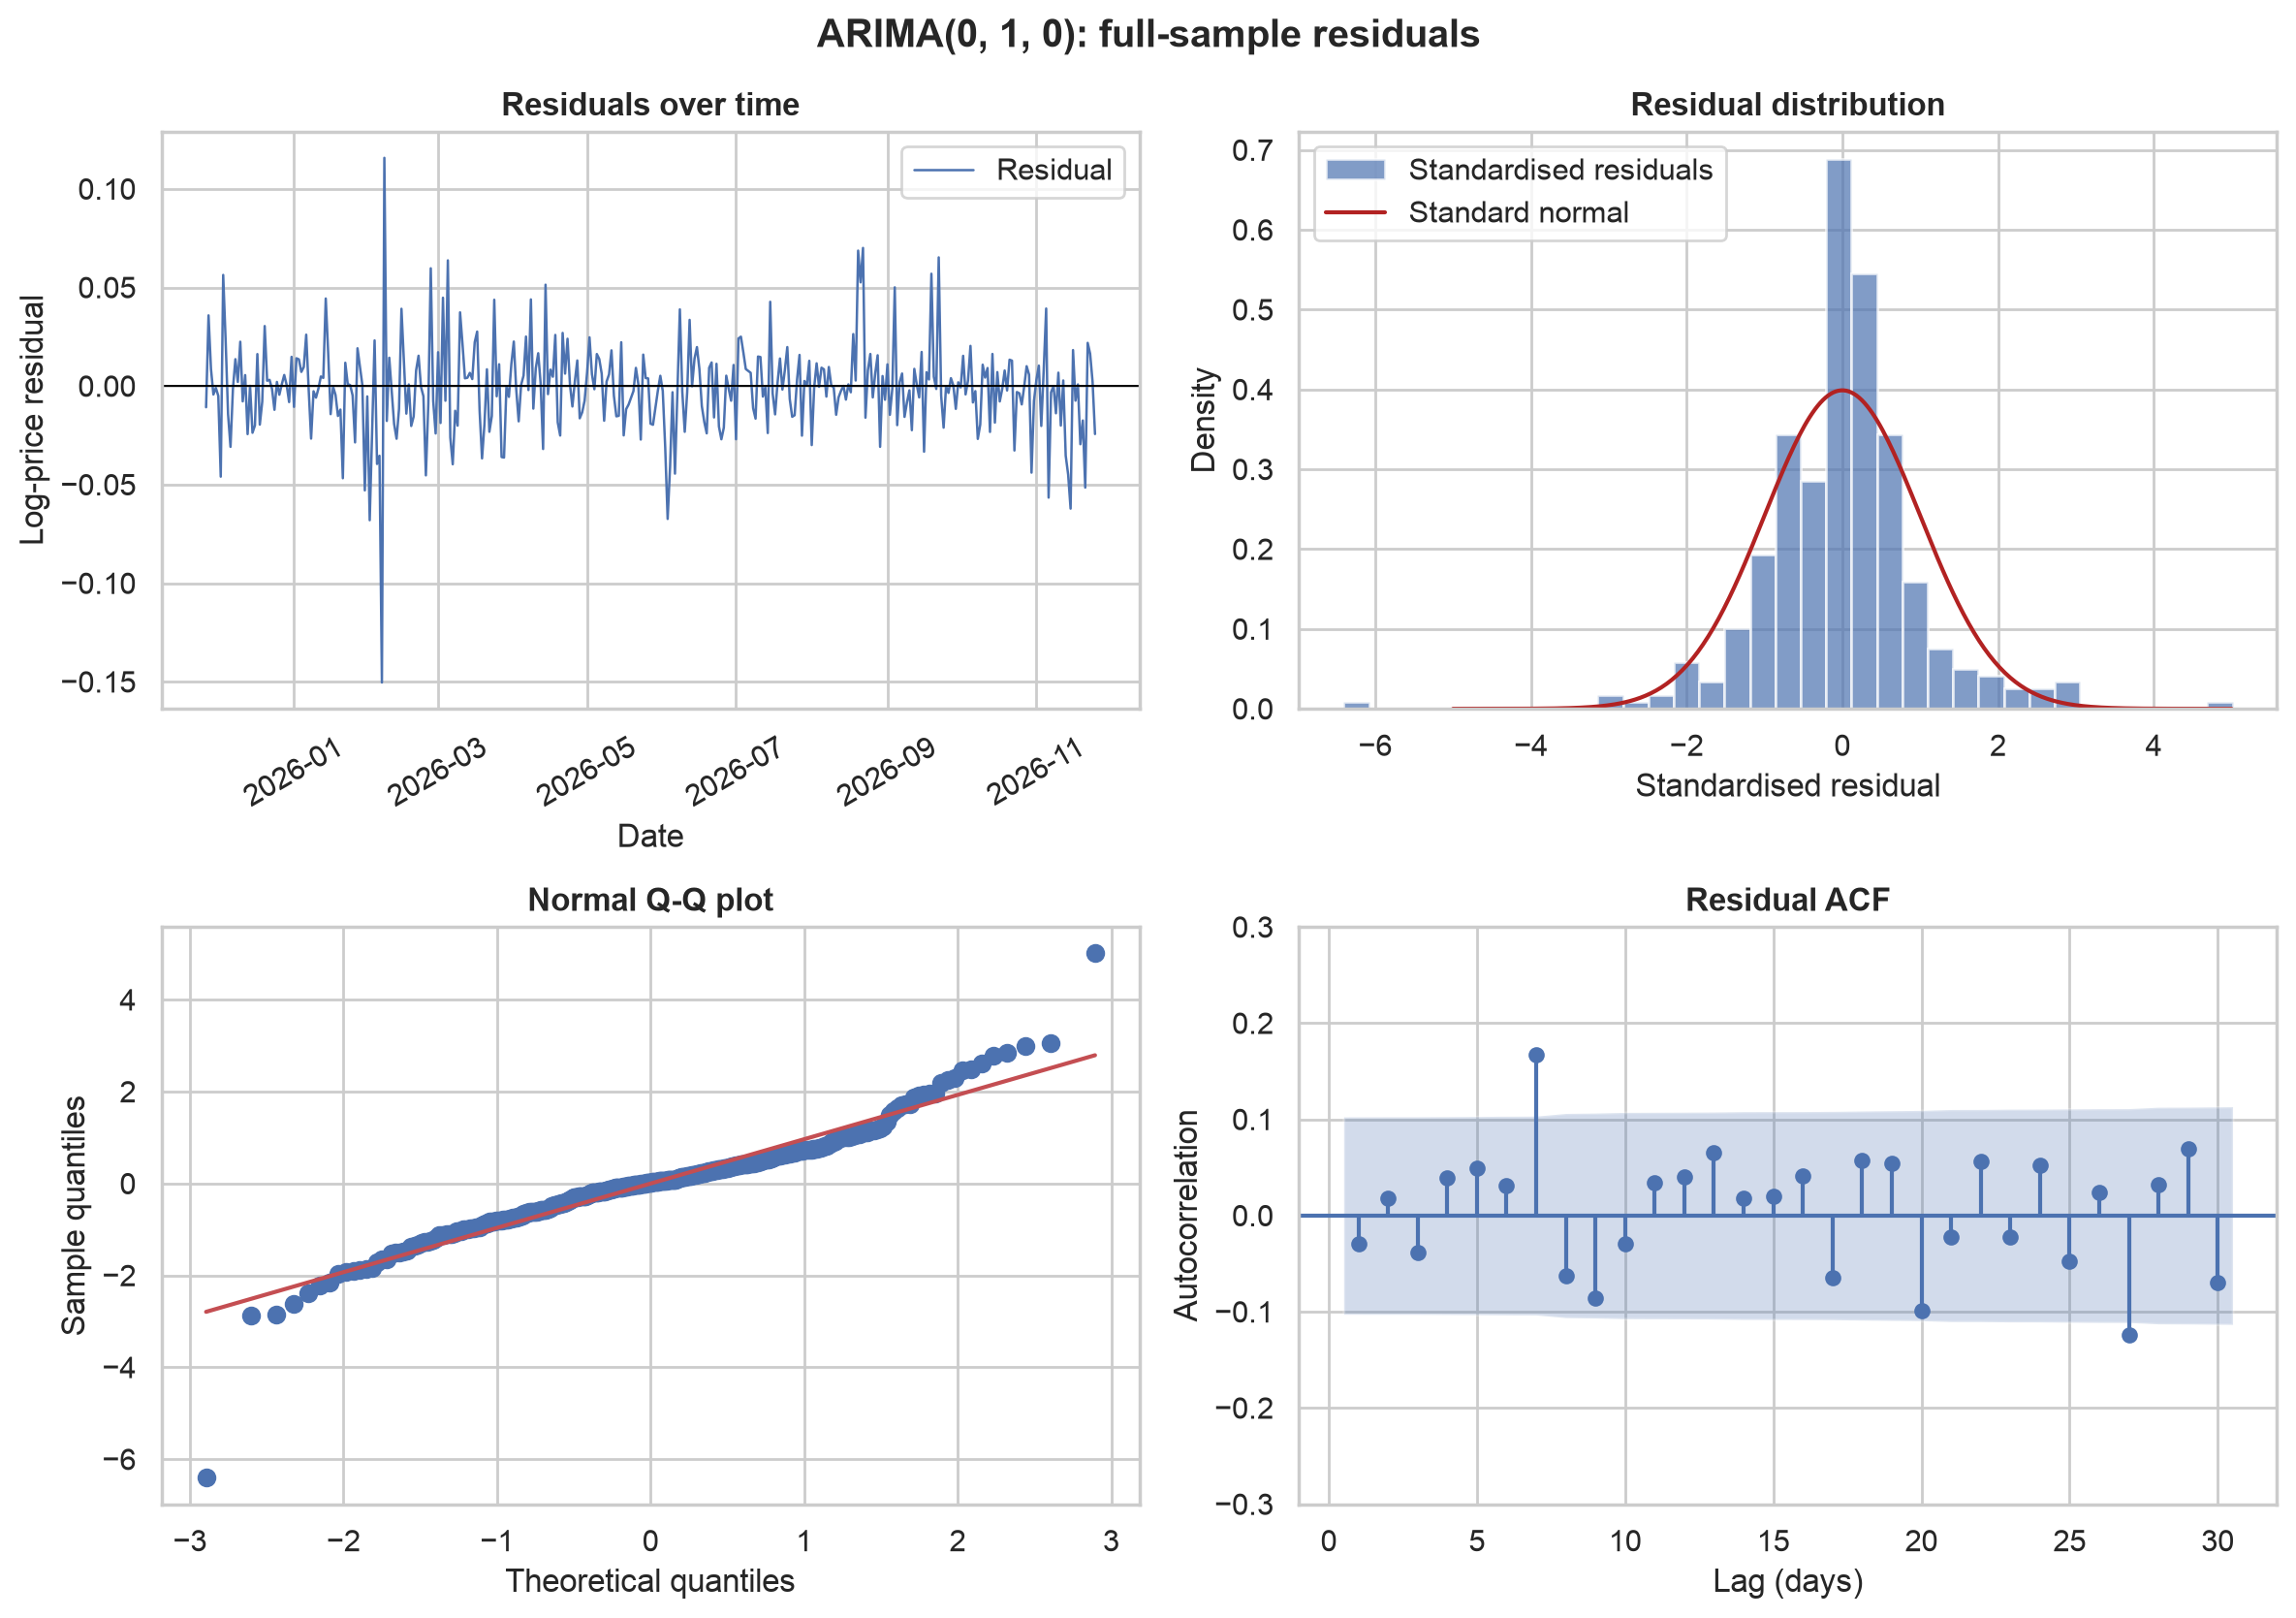
\includegraphics[width=\linewidth,height=0.78\textheight,keepaspectratio]{figures/model_diagnostics_full_sample.png}
\caption{Residual diagnostics, ARIMA(0, 1, 0), full sample}
\end{figure}

\begin{figure}[H]
\centering
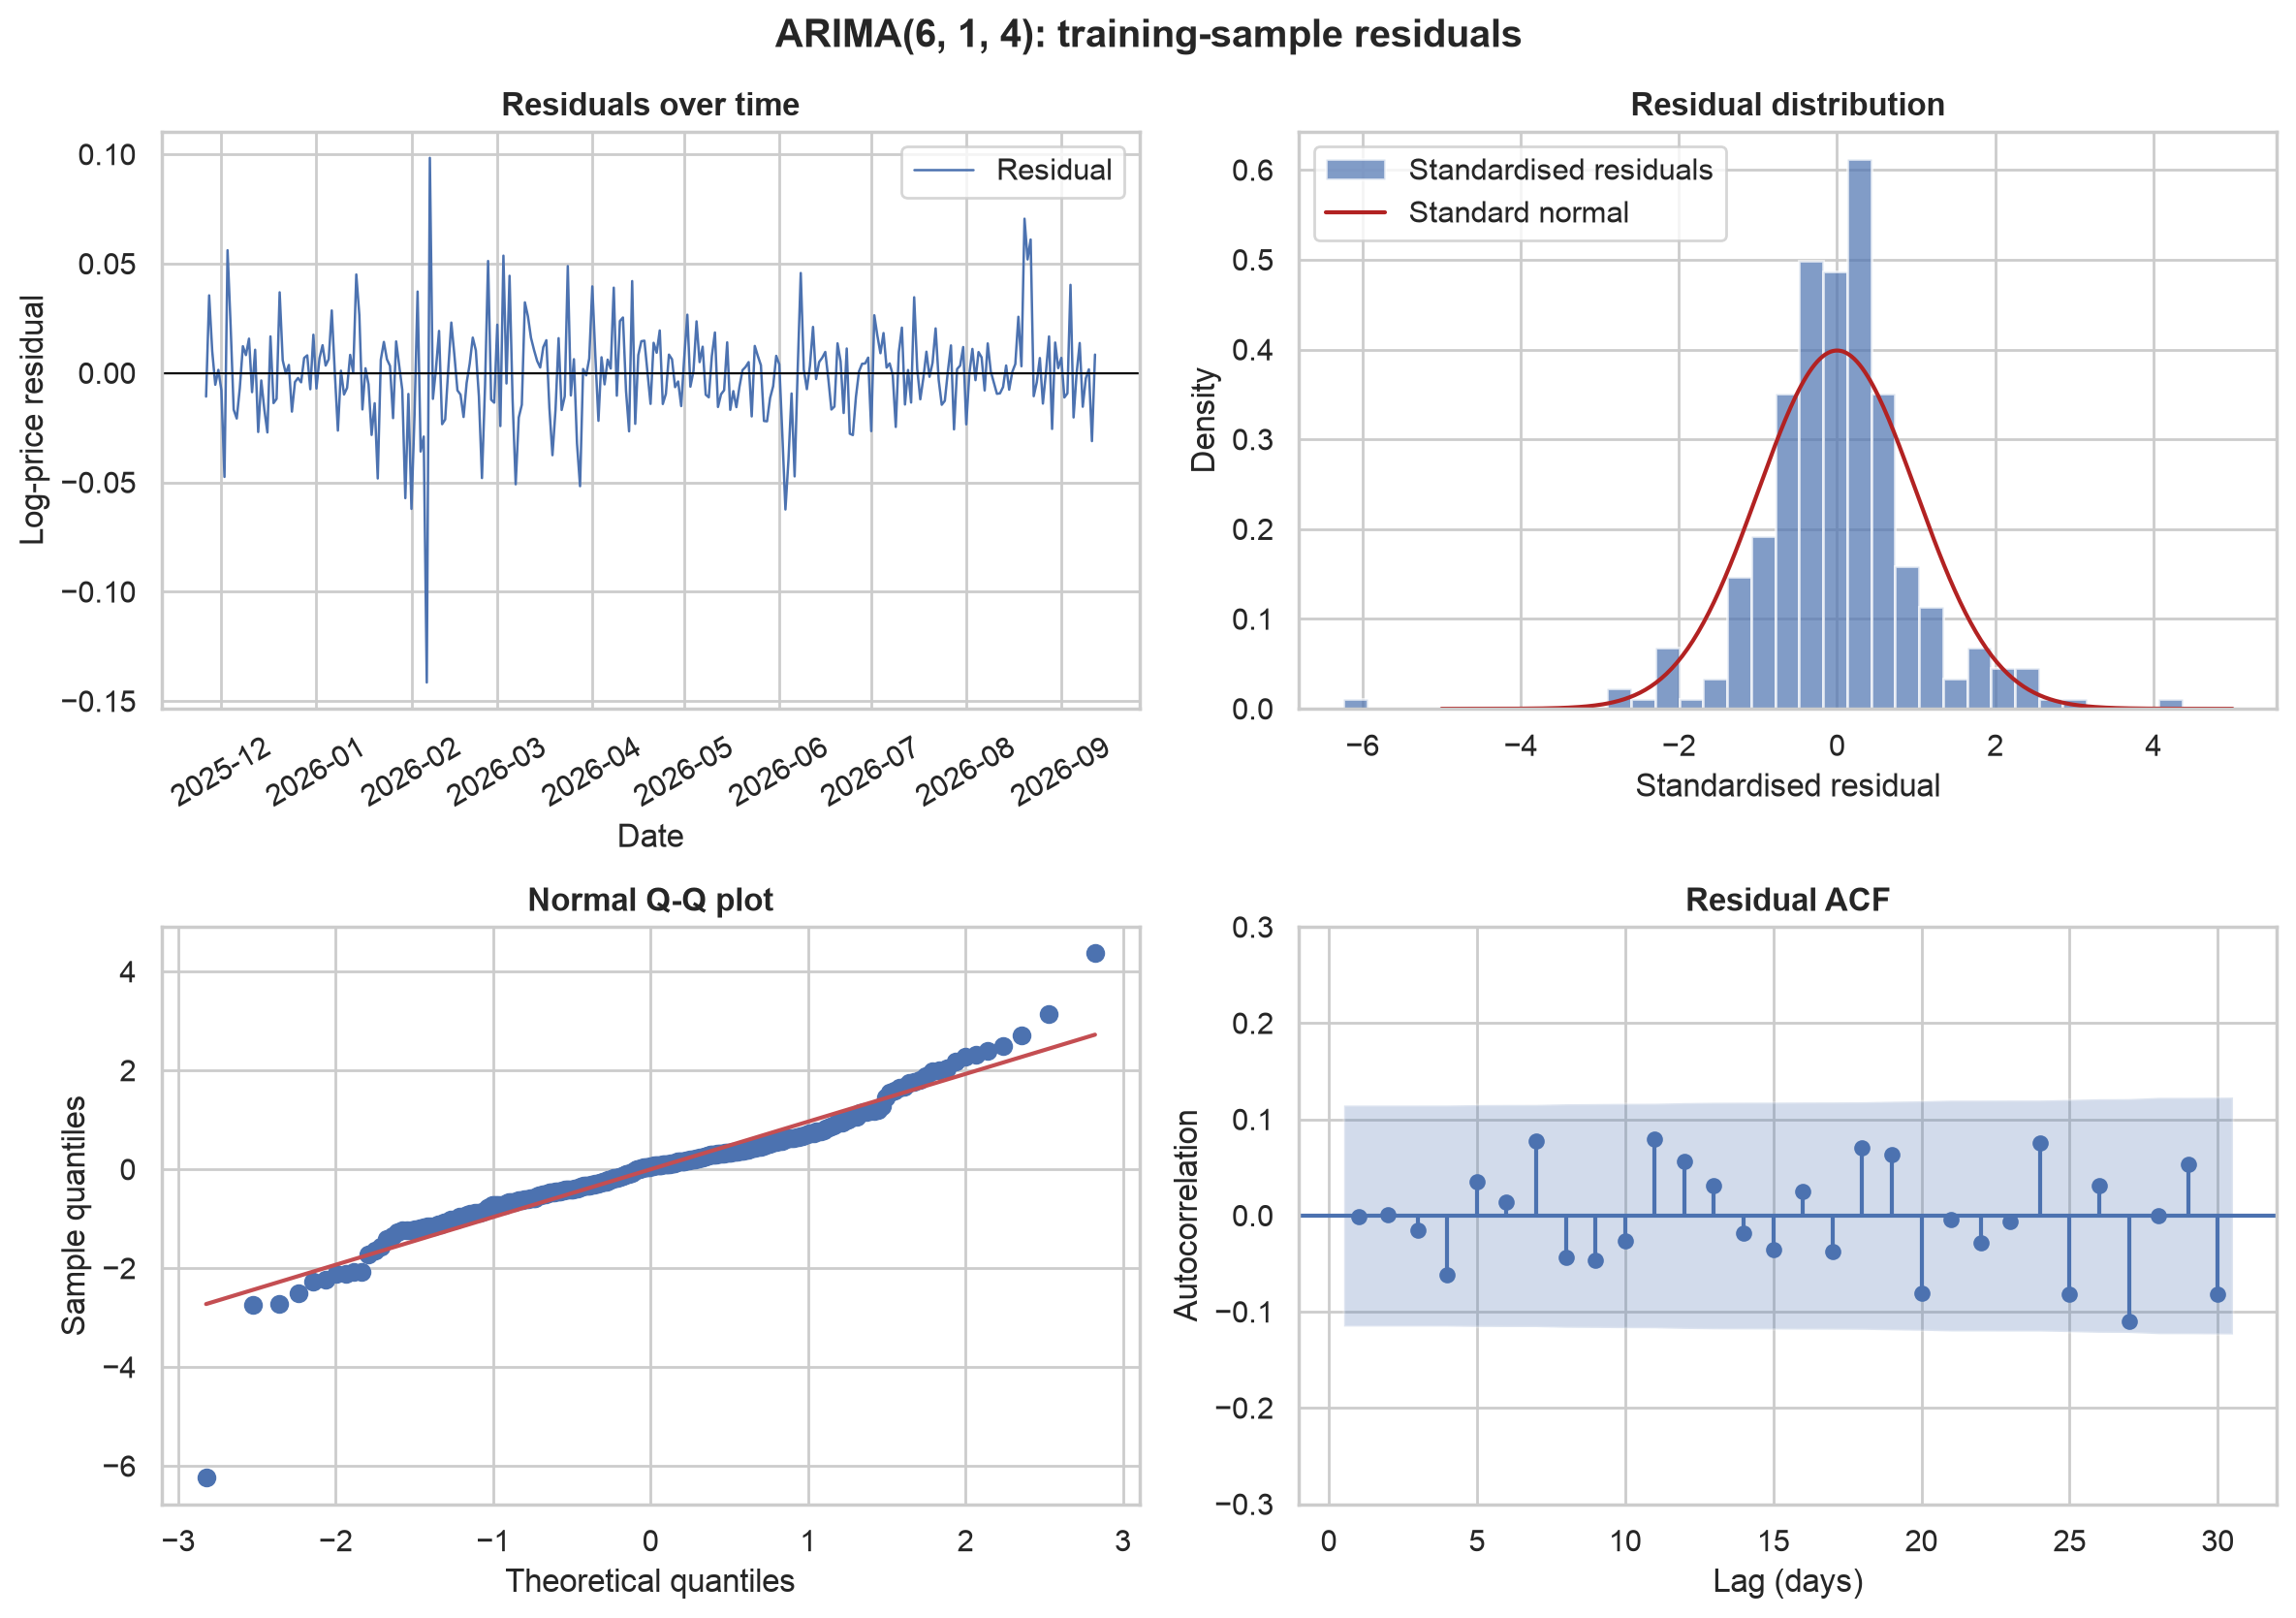
\includegraphics[width=\linewidth,height=0.78\textheight,keepaspectratio]{figures/sensitivity_diagnostics.png}
\caption{Residual diagnostics, sensitivity model ARIMA(6, 1, 4), training sample}
\end{figure}

\begin{figure}[H]
\centering
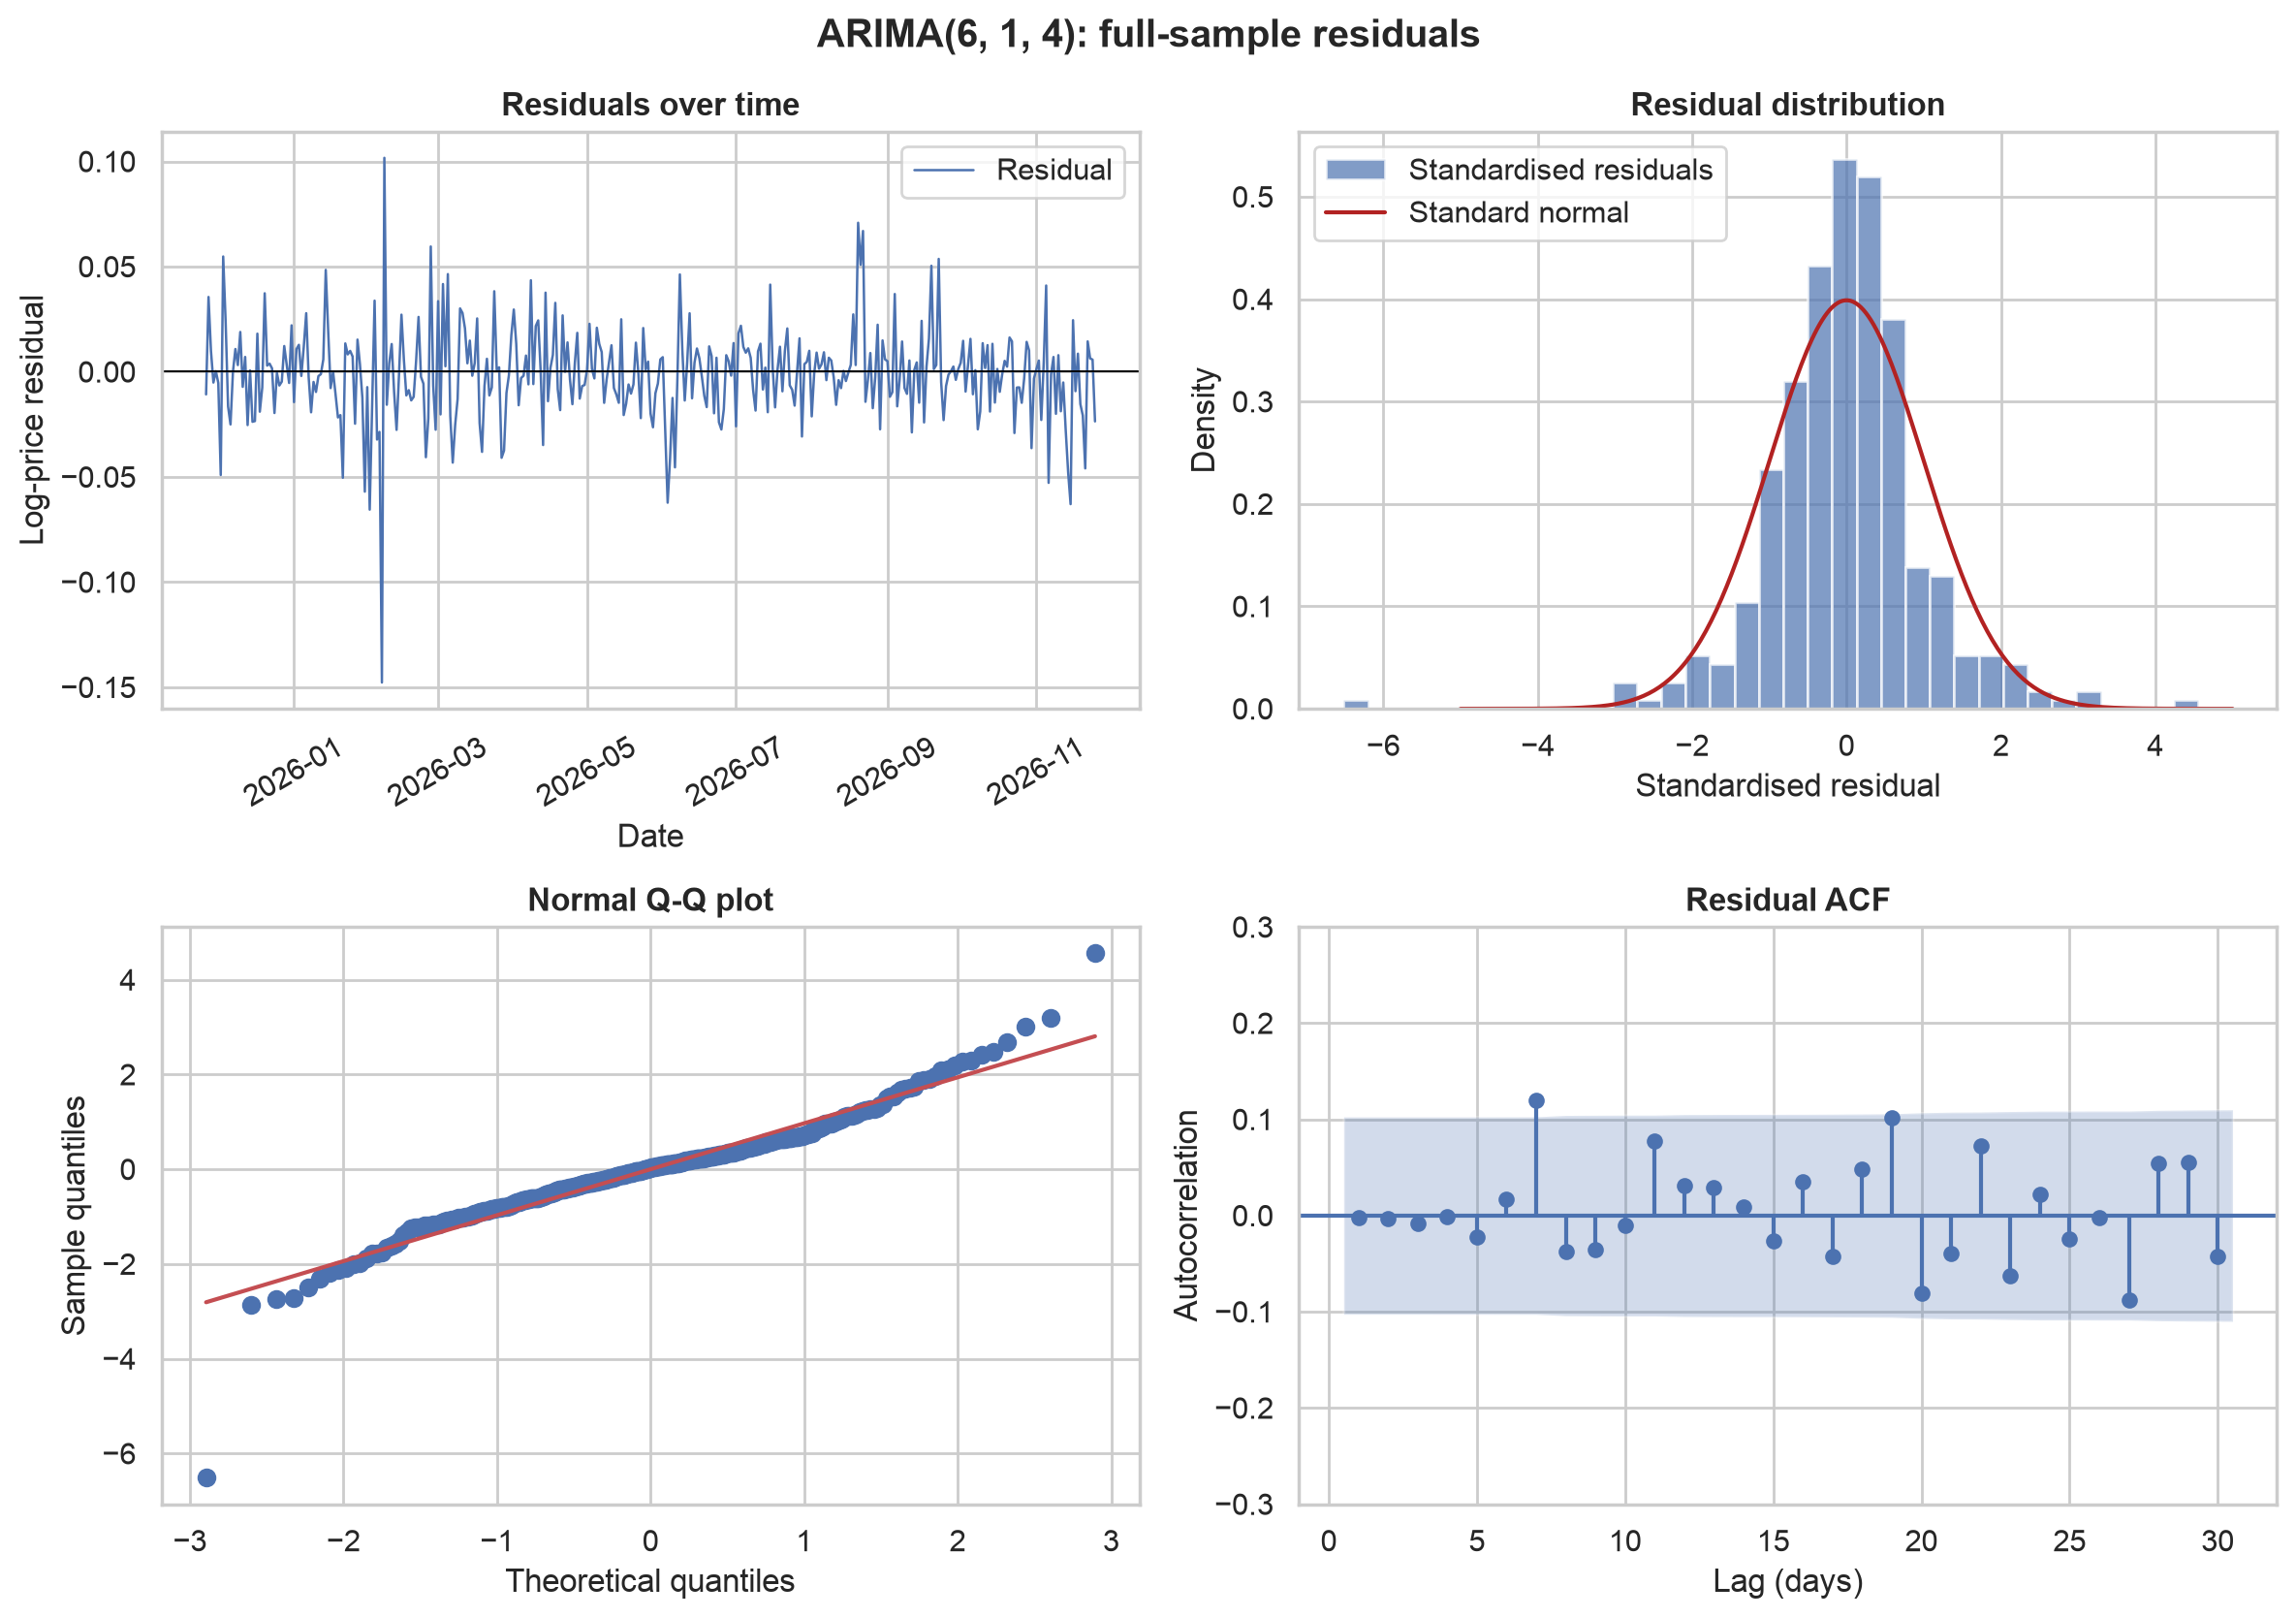
\includegraphics[width=\linewidth,height=0.78\textheight,keepaspectratio]{figures/sensitivity_diagnostics_full_sample.png}
\caption{Residual diagnostics, sensitivity model ARIMA(6, 1, 4), full sample}
\end{figure}

\begin{table}[H]
\centering
\caption{Residual tests (LB(10) is undefined when p + q = 10)}
\footnotesize
\setlength{\tabcolsep}{4pt}
\begin{adjustbox}{max width=\linewidth}
\begin{tabular}{lrrrrrr}
\toprule
\textbf{Model and sample} & \textbf{LB(10) p} & \textbf{LB(20) p} & \textbf{Mean=0 p} & \textbf{Excess kurt.} & \textbf{Jarque-Bera p} & \textbf{ARCH LM p} \\
\midrule
ARIMA(0, 1, 0) training & 0.163 & 0.199 & 0.740 & 7.23 & \textless{}0.001 & \textless{}0.001 \\
ARIMA(0, 1, 0) full & 0.059 & 0.084 & 0.381 & 6.39 & \textless{}0.001 & \textless{}0.001 \\
ARIMA(6, 1, 4) training & n/a & 0.173 & 0.745 & 6.30 & \textless{}0.001 & \textless{}0.001 \\
ARIMA(6, 1, 4) full & n/a & 0.046 & 0.395 & 6.07 & \textless{}0.001 & \textless{}0.001 \\
\bottomrule
\end{tabular}
\end{adjustbox}
\end{table}

For ARIMA(0, 1, 0), Ljung-Box does not reject at 5\% on either sample, and the mean residual is not distinguishable from zero. The full-sample result is borderline (lag 10 p = 0.059), and the ACF shows an isolated lag-7 spike, so weak dependence cannot be excluded. The residuals are not independent, identically distributed Gaussian noise: Jarque-Bera strongly rejects normality, and both the ARCH test (Engle, 1982) and the autocorrelation of squared residuals show volatility clustering. The model is therefore acceptable for the linear mean, but inadequate as a description of risk. Constant-variance Gaussian intervals will be too narrow in turbulent periods and too wide in calm ones.

\section{Seven-Day Forecast Results}

ARIMA(0, 1, 0) was refitted to all 366 observations. The forecast origin is 2026-11-25 at \$59,742.21.

\begin{table}[H]
\centering
\caption{Seven-day forecast}
\footnotesize
\setlength{\tabcolsep}{4pt}
\begin{adjustbox}{max width=\linewidth}
\begin{tabular}{rrrrrl}
\toprule
\textbf{Date} & \textbf{Forecast (USD)} & \textbf{Lower 95\%} & \textbf{Upper 95\%} & \textbf{Daily change} & \textbf{Direction} \\
\midrule
2026-11-26 & \$59,742.21 & \$57,075.64 & \$62,533.36 & 0.00\% & Neutral \\
2026-11-27 & \$59,742.21 & \$56,006.28 & \$63,727.35 & 0.00\% & Neutral \\
2026-11-28 & \$59,742.21 & \$55,199.33 & \$64,658.96 & 0.00\% & Neutral \\
2026-11-29 & \$59,742.21 & \$54,528.09 & \$65,454.92 & 0.00\% & Neutral \\
2026-11-30 & \$59,742.21 & \$53,943.48 & \$66,164.29 & 0.00\% & Neutral \\
2026-12-01 & \$59,742.21 & \$53,420.34 & \$66,812.22 & 0.00\% & Neutral \\
2026-12-02 & \$59,742.21 & \$52,943.75 & \$67,413.66 & 0.00\% & Neutral \\
\bottomrule
\end{tabular}
\end{adjustbox}
\end{table}

\begin{figure}[H]
\centering
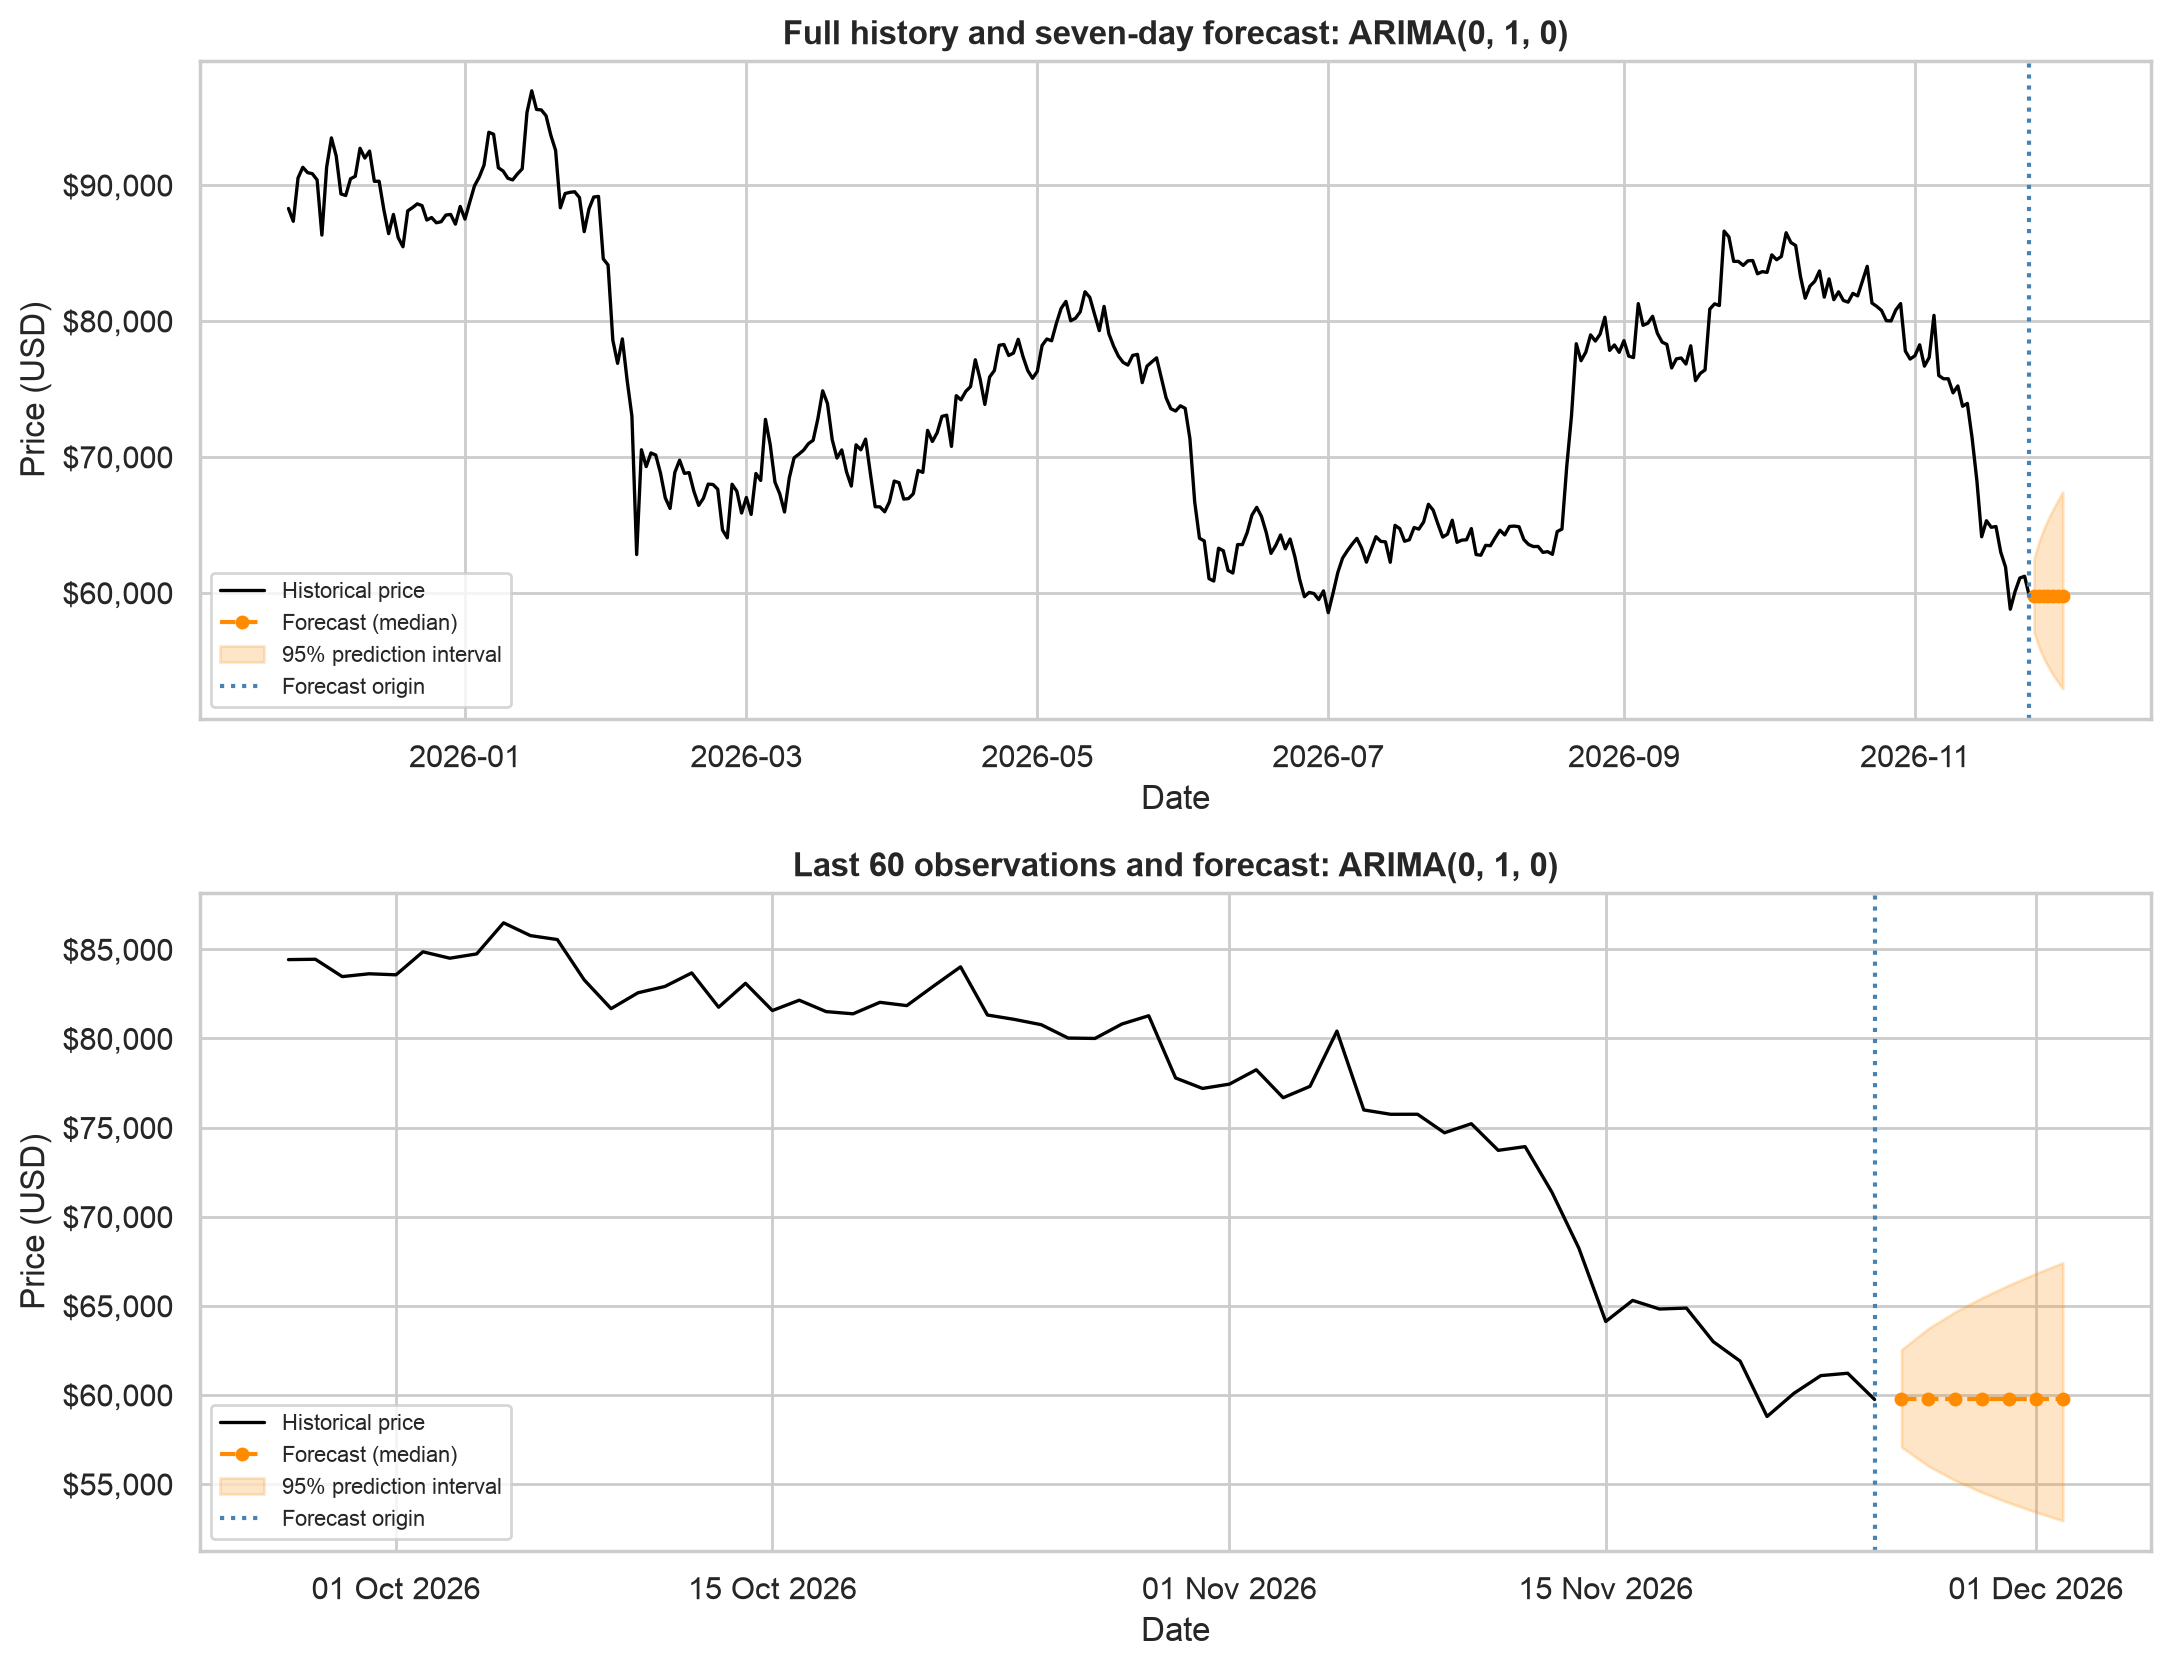
\includegraphics[width=\linewidth,height=0.78\textheight,keepaspectratio]{figures/seven_day_forecast.png}
\caption{Historical price, seven-day forecast and 95\% prediction interval}
\end{figure}

Classification: Neutral. A daily change smaller than 0.10\% in absolute value is labelled Neutral, and a seven-day change smaller than 1\% is classed as Neutral overall (larger rises are Bullish, larger falls Bearish). These thresholds are reporting conventions chosen for this study, not statistical tests.

The expected change is 0.00\% and there are no daily fluctuations in the point forecast, because a driftless random walk assigns the same median to every future day. Actual prices will fluctuate. The interval widens from \$5,457.73 on day one to \$14,469.91 on day seven (24.2\% of the forecast). The log-normal mean on day seven is \$59,855.81; its excess over the median arises from the variance correction and is not a directional signal.

\begin{table}[H]
\centering
\caption{Sensitivity analysis: forecast from ARIMA(6, 1, 4) (not the selected model)}
\footnotesize
\setlength{\tabcolsep}{4pt}
\begin{adjustbox}{max width=\linewidth}
\begin{tabular}{rrrrrl}
\toprule
\textbf{Date} & \textbf{Forecast (USD)} & \textbf{Lower 95\%} & \textbf{Upper 95\%} & \textbf{Daily change} & \textbf{Direction} \\
\midrule
2026-11-26 & \$59,419.16 & \$56,876.41 & \$62,075.60 & -0.54\% & Down \\
2026-11-27 & \$58,839.05 & \$55,379.32 & \$62,514.92 & -0.98\% & Down \\
2026-11-28 & \$59,038.48 & \$54,824.69 & \$63,576.15 & 0.34\% & Up \\
2026-11-29 & \$58,815.86 & \$54,042.99 & \$64,010.25 & -0.38\% & Down \\
2026-11-30 & \$58,948.47 & \$53,531.90 & \$64,913.11 & 0.23\% & Up \\
2026-12-01 & \$59,425.16 & \$53,308.31 & \$66,243.89 & 0.81\% & Up \\
2026-12-02 & \$59,274.21 & \$52,564.02 & \$66,841.01 & -0.25\% & Down \\
\bottomrule
\end{tabular}
\end{adjustbox}
\end{table}

The sensitivity model gives alternating daily moves and a seven-day change of -0.78\% (to \$59,274.21), which is also Neutral under the same threshold. Its departure from the flat forecast is small relative to the interval width, so the overall conclusion does not depend on the root screen, although the day-to-day directions do.

\section{Discussion}

The expected direction is neutral. This is a result rather than a failure of the procedure: lags 1 to 6 carry little linear information, the more complex candidates were either inadmissible or no better in validation, and no alternative showed a statistically significant test improvement over the naive forecast.

The forecast is not a statistically meaningful directional prediction. The model does not predict that the price will stay at \$59,742.21; it states that, given only past prices, upward and downward moves in log price are treated as symmetric around today's value. A seven-day outcome anywhere between about \$52,943.75 and \$67,413.66 would be consistent with the fitted model, and outcomes outside that range remain possible, particularly given heavy tails and the recent rise in rolling dispersion.

The main strengths of the approach are its transparency, chronological validation, explicit benchmarks and honest intervals relative to a point forecast. Its main weakness is that it offers no skill beyond the naive method. These forecasts are statistical outputs for academic assessment and are not investment advice.

\section{Limitations}

\begin{itemize}
  \item One year of data covers few market regimes; results may not generalise.
  \item ARIMA is linear and univariate. It excludes trading volume, other markets, news and on-chain variables.
  \item Residual variance is not constant and tails are heavy, so Gaussian intervals are approximate.
  \item The root screen was added after initial results were seen, so model selection was not fully blind.
  \item The validation (58 days) and test (74 days) samples are short, giving low statistical power; seven-day forecasts also overlap.
  \item Differences between candidate models are small and could reverse with a different window.
  \item The source does not fully document how its market price is aggregated or whether values are revised.
  \item The lag-7 correlation was not modelled with a seasonal term. SARIMA and GARCH-type models are natural extensions and should be assessed on new data.
\end{itemize}

\section{Conclusion}

Using genuine Blockchain.com data for 2025-11-25 to 2026-11-25, the evidence supports one difference of log price and selects ARIMA(0, 1, 0) under the stated screen. The seven-day forecast is Neutral, with a median of \$59,742.21 and a seventh-day 95\% interval of \$52,943.75 to \$67,413.66. Out-of-sample accuracy equals that of the naive forecast. ARIMA therefore provides a disciplined baseline and a measure of uncertainty, but no demonstrated ability to predict the direction of Bitcoin over the coming week.

Reproducibility: run run\_pipeline.py on the saved snapshot; package versions are listed in requirements.txt (Python 3.14.3, statsmodels 0.15.0, pmdarima 2.1.1).

\clearpage
\section*{References}
\addcontentsline{toc}{section}{References}

\begin{hangparas}{2.5em}{1}
\raggedright
Akaike, H. (1974) `A new look at the statistical model identification', IEEE Transactions on Automatic Control, 19(6), pp. 716-723. doi:10.1109/TAC.1974.1100705.

Blockchain.com (2026) Market Price (USD) chart. Available at: \url{https://www.blockchain.com/ko/charts/market-price} (data retrieved 25 November 2026).

Blockchain.com (2026) Charts and statistics API. Available at: \url{https://www.blockchain.com/explorer/api/charts_api}.

Box, G.E.P., Jenkins, G.M., Reinsel, G.C. and Ljung, G.M. (2015) Time Series Analysis: Forecasting and Control. 5th edn. Hoboken: Wiley.

Coinbase (2026) Exchange API: product candles, BTC-USD. Available at: \url{https://api.exchange.coinbase.com/products/BTC-USD/candles} (used for verification only).

Cont, R. (2001) `Empirical properties of asset returns: stylized facts and statistical issues', Quantitative Finance, 1(2), pp. 223-236. doi:10.1080/713665670.

Dickey, D.A. and Fuller, W.A. (1979) `Distribution of the estimators for autoregressive time series with a unit root', Journal of the American Statistical Association, 74(366), pp. 427-431. doi:10.1080/01621459.1979.10482531.

Diebold, F.X. and Mariano, R.S. (1995) `Comparing predictive accuracy', Journal of Business \& Economic Statistics, 13(3), pp. 253-263. doi:10.1080/07350015.1995.10524599.

Engle, R.F. (1982) `Autoregressive conditional heteroscedasticity with estimates of the variance of United Kingdom inflation', Econometrica, 50(4), pp. 987-1007. doi:10.2307/1912773.

Fama, E.F. (1970) `Efficient capital markets: a review of theory and empirical work', The Journal of Finance, 25(2), pp. 383-417. doi:10.2307/2325486.

Harvey, D., Leybourne, S. and Newbold, P. (1997) `Testing the equality of prediction mean squared errors', International Journal of Forecasting, 13(2), pp. 281-291. doi:10.1016/S0169-2070(96)00719-4.

Hyndman, R.J. and Khandakar, Y. (2008) `Automatic time series forecasting: the forecast package for R', Journal of Statistical Software, 27(3). doi:10.18637/jss.v027.i03.

Hyndman, R.J. and Koehler, A.B. (2006) `Another look at measures of forecast accuracy', International Journal of Forecasting, 22(4), pp. 679-688. doi:10.1016/j.ijforecast.2006.03.001.

Kwiatkowski, D., Phillips, P.C.B., Schmidt, P. and Shin, Y. (1992) `Testing the null hypothesis of stationarity against the alternative of a unit root', Journal of Econometrics, 54(1-3), pp. 159-178. doi:10.1016/0304-4076(92)90104-Y.

Ljung, G.M. and Box, G.E.P. (1978) `On a measure of lack of fit in time series models', Biometrika, 65(2), pp. 297-303. doi:10.1093/biomet/65.2.297.

Meese, R.A. and Rogoff, K. (1983) `Empirical exchange rate models of the seventies: do they fit out of sample?', Journal of International Economics, 14(1-2), pp. 3-24. doi:10.1016/0022-1996(83)90017-X.

pmdarima developers (2026) pmdarima documentation. Available at: \url{https://alkaline-ml.com/pmdarima/}.

Said, S.E. and Dickey, D.A. (1984) `Testing for unit roots in autoregressive-moving average models of unknown order', Biometrika, 71(3), pp. 599-607. doi:10.1093/biomet/71.3.599.

Schwarz, G. (1978) `Estimating the dimension of a model', The Annals of Statistics, 6(2), pp. 461-464. doi:10.1214/aos/1176344136.

Seabold, S. and Perktold, J. (2010) `Statsmodels: econometric and statistical modeling with Python', Proceedings of the 9th Python in Science Conference, pp. 92-96. doi:10.25080/Majora-92bf1922-011.

statsmodels developers (2026) ARIMA documentation. Available at: \url{https://www.statsmodels.org/stable/generated/statsmodels.tsa.arima.model.ARIMA.html}.

Tashman, L.J. (2000) `Out-of-sample tests of forecasting accuracy: an analysis and review', International Journal of Forecasting, 16(4), pp. 437-450. doi:10.1016/S0169-2070(00)00065-0.
\end{hangparas}

\clearpage
\appendix
\section{Test-Period Predictions}

{\small
\begin{longtable}{rrrrr}
\caption{One-step walk-forward predictions, ARIMA(0, 1, 0)}\\
\toprule
\textbf{Date} & \textbf{Actual} & \textbf{Predicted} & \textbf{Absolute error} & \textbf{Percentage error} \\
\midrule
\endfirsthead
\toprule
\textbf{Date} & \textbf{Actual} & \textbf{Predicted} & \textbf{Absolute error} & \textbf{Percentage error} \\
\midrule
\endhead
\bottomrule
\endfoot
2026-09-13 & \$77,273.07 & \$77,209.87 & \$63.20 & 0.08\% \\
2026-09-14 & \$76,829.51 & \$77,273.07 & \$443.56 & 0.58\% \\
2026-09-15 & \$78,169.72 & \$76,829.51 & \$1,340.21 & 1.71\% \\
2026-09-16 & \$75,609.19 & \$78,169.72 & \$2,560.53 & 3.39\% \\
2026-09-17 & \$76,141.53 & \$75,609.19 & \$532.34 & 0.70\% \\
2026-09-18 & \$76,395.02 & \$76,141.53 & \$253.49 & 0.33\% \\
2026-09-19 & \$80,872.23 & \$76,395.02 & \$4,477.21 & 5.54\% \\
2026-09-20 & \$81,256.73 & \$80,872.23 & \$384.50 & 0.47\% \\
2026-09-21 & \$81,136.20 & \$81,256.73 & \$120.53 & 0.15\% \\
2026-09-22 & \$86,607.63 & \$81,136.20 & \$5,471.43 & 6.32\% \\
2026-09-23 & \$86,184.81 & \$86,607.63 & \$422.82 & 0.49\% \\
2026-09-24 & \$84,384.61 & \$86,184.81 & \$1,800.20 & 2.13\% \\
2026-09-25 & \$84,380.26 & \$84,384.61 & \$4.35 & 0.01\% \\
2026-09-26 & \$84,087.22 & \$84,380.26 & \$293.04 & 0.35\% \\
2026-09-27 & \$84,423.31 & \$84,087.22 & \$336.09 & 0.40\% \\
2026-09-28 & \$84,443.93 & \$84,423.31 & \$20.62 & 0.02\% \\
2026-09-29 & \$83,471.07 & \$84,443.93 & \$972.86 & 1.17\% \\
2026-09-30 & \$83,629.12 & \$83,471.07 & \$158.05 & 0.19\% \\
2026-10-01 & \$83,570.96 & \$83,629.12 & \$58.16 & 0.07\% \\
2026-10-02 & \$84,862.44 & \$83,570.96 & \$1,291.48 & 1.52\% \\
2026-10-03 & \$84,502.85 & \$84,862.44 & \$359.59 & 0.43\% \\
2026-10-04 & \$84,743.72 & \$84,502.85 & \$240.87 & 0.28\% \\
2026-10-05 & \$86,488.03 & \$84,743.72 & \$1,744.31 & 2.02\% \\
2026-10-06 & \$85,770.88 & \$86,488.03 & \$717.15 & 0.84\% \\
2026-10-07 & \$85,549.02 & \$85,770.88 & \$221.86 & 0.26\% \\
2026-10-08 & \$83,285.33 & \$85,549.02 & \$2,263.69 & 2.72\% \\
2026-10-09 & \$81,672.90 & \$83,285.33 & \$1,612.43 & 1.97\% \\
2026-10-10 & \$82,561.72 & \$81,672.90 & \$888.82 & 1.08\% \\
2026-10-11 & \$82,916.77 & \$82,561.72 & \$355.05 & 0.43\% \\
2026-10-12 & \$83,677.37 & \$82,916.77 & \$760.60 & 0.91\% \\
2026-10-13 & \$81,751.90 & \$83,677.37 & \$1,925.47 & 2.36\% \\
2026-10-14 & \$83,093.75 & \$81,751.90 & \$1,341.85 & 1.61\% \\
2026-10-15 & \$81,566.64 & \$83,093.75 & \$1,527.11 & 1.87\% \\
2026-10-16 & \$82,145.34 & \$81,566.64 & \$578.70 & 0.70\% \\
2026-10-17 & \$81,505.93 & \$82,145.34 & \$639.41 & 0.78\% \\
2026-10-18 & \$81,382.82 & \$81,505.93 & \$123.11 & 0.15\% \\
2026-10-19 & \$82,027.16 & \$81,382.82 & \$644.34 & 0.79\% \\
2026-10-20 & \$81,842.66 & \$82,027.16 & \$184.50 & 0.23\% \\
2026-10-21 & \$82,942.91 & \$81,842.66 & \$1,100.25 & 1.33\% \\
2026-10-22 & \$84,018.76 & \$82,942.91 & \$1,075.85 & 1.28\% \\
2026-10-23 & \$81,315.73 & \$84,018.76 & \$2,703.03 & 3.32\% \\
2026-10-24 & \$81,069.69 & \$81,315.73 & \$246.04 & 0.30\% \\
2026-10-25 & \$80,771.90 & \$81,069.69 & \$297.79 & 0.37\% \\
2026-10-26 & \$80,022.79 & \$80,771.90 & \$749.11 & 0.94\% \\
2026-10-27 & \$80,000.34 & \$80,022.79 & \$22.45 & 0.03\% \\
2026-10-28 & \$80,808.65 & \$80,000.34 & \$808.31 & 1.00\% \\
2026-10-29 & \$81,275.48 & \$80,808.65 & \$466.83 & 0.57\% \\
2026-10-30 & \$77,782.24 & \$81,275.48 & \$3,493.24 & 4.49\% \\
2026-10-31 & \$77,195.55 & \$77,782.24 & \$586.69 & 0.76\% \\
2026-11-01 & \$77,437.09 & \$77,195.55 & \$241.54 & 0.31\% \\
2026-11-02 & \$78,242.98 & \$77,437.09 & \$805.89 & 1.03\% \\
2026-11-03 & \$76,675.03 & \$78,242.98 & \$1,567.95 & 2.04\% \\
2026-11-04 & \$77,313.17 & \$76,675.03 & \$638.14 & 0.83\% \\
2026-11-05 & \$80,413.00 & \$77,313.17 & \$3,099.83 & 3.85\% \\
2026-11-06 & \$75,988.30 & \$80,413.00 & \$4,424.70 & 5.82\% \\
2026-11-07 & \$75,744.59 & \$75,988.30 & \$243.71 & 0.32\% \\
2026-11-08 & \$75,746.54 & \$75,744.59 & \$1.95 & 0.00\% \\
2026-11-09 & \$74,707.15 & \$75,746.54 & \$1,039.39 & 1.39\% \\
2026-11-10 & \$75,215.41 & \$74,707.15 & \$508.26 & 0.68\% \\
2026-11-11 & \$73,722.16 & \$75,215.41 & \$1,493.25 & 2.03\% \\
2026-11-12 & \$73,930.74 & \$73,722.16 & \$208.58 & 0.28\% \\
2026-11-13 & \$71,365.77 & \$73,930.74 & \$2,564.97 & 3.59\% \\
2026-11-14 & \$68,232.31 & \$71,365.77 & \$3,133.46 & 4.59\% \\
2026-11-15 & \$64,119.34 & \$68,232.31 & \$4,112.97 & 6.41\% \\
2026-11-16 & \$65,300.42 & \$64,119.34 & \$1,181.08 & 1.81\% \\
2026-11-17 & \$64,817.91 & \$65,300.42 & \$482.51 & 0.74\% \\
2026-11-18 & \$64,871.15 & \$64,817.91 & \$53.24 & 0.08\% \\
2026-11-19 & \$62,984.54 & \$64,871.15 & \$1,886.61 & 3.00\% \\
2026-11-20 & \$61,893.71 & \$62,984.54 & \$1,090.83 & 1.76\% \\
2026-11-21 & \$58,786.67 & \$61,893.71 & \$3,107.04 & 5.29\% \\
2026-11-22 & \$60,088.31 & \$58,786.67 & \$1,301.64 & 2.17\% \\
2026-11-23 & \$61,081.74 & \$60,088.31 & \$993.43 & 1.63\% \\
2026-11-24 & \$61,214.41 & \$61,081.74 & \$132.67 & 0.22\% \\
2026-11-25 & \$59,742.21 & \$61,214.41 & \$1,472.20 & 2.46\% \\
\end{longtable}
}

\clearpage
\section{Python Source Code}

The analysis is implemented in Python. The listings below are the files that produce the data, figures and results in this report.

\subsection{\texttt{run\_pipeline.py}}
\lstinputlisting{code/run_pipeline.py}

\subsection{\texttt{src/config.py}}
\lstinputlisting{code/src_config.py}

\subsection{\texttt{src/data\_collection.py}}
\lstinputlisting{code/src_data_collection.py}

\subsection{\texttt{src/preprocessing.py}}
\lstinputlisting{code/src_preprocessing.py}

\subsection{\texttt{src/exploratory\_analysis.py}}
\lstinputlisting{code/src_exploratory_analysis.py}

\subsection{\texttt{src/stationarity.py}}
\lstinputlisting{code/src_stationarity.py}

\subsection{\texttt{src/arima\_model.py}}
\lstinputlisting{code/src_arima_model.py}

\subsection{\texttt{src/forecasting.py}}
\lstinputlisting{code/src_forecasting.py}

\subsection{\texttt{src/cross\_check.py}}
\lstinputlisting{code/src_cross_check.py}

\end{document}
